% Informe completo de reproducción y réplica experimental del paper:
% «A Fast Wait-Free Solution to Read-Reclaim Races in Reference Counting» (Euro-Par 2024)
% Compilación (desde replica/informe_completo/):
%   pdflatex informe_replica_ultra9.tex && bibtex informe_replica_ultra9 && pdflatex informe_replica_ultra9.tex && pdflatex informe_replica_ultra9.tex
\documentclass[11pt,a4paper]{article}
\usepackage[utf8]{inputenc}
\usepackage[T1]{fontenc}
\usepackage[spanish,es-noshorthands,es-nodecimaldot,es-tabla]{babel}
\spanishplainpercent
\usepackage{geometry}
\geometry{margin=2.1cm}
\usepackage{booktabs,tabularx,array,longtable,multirow}
\usepackage{graphicx,float}
\usepackage{amsmath,amssymb,pifont}
\usepackage{xcolor}
\usepackage{caption}
\usepackage{cite}
\usepackage{xurl}
\usepackage{hyperref}

% Paleta sobria (coherente con las diapositivas del repositorio)
\definecolor{tinta}{HTML}{1B2430}
\definecolor{gris}{HTML}{5B6573}
\definecolor{acento}{HTML}{C8551F}
\definecolor{azul}{HTML}{1F5FA8}
\definecolor{ok}{HTML}{1B7F3B}
\definecolor{mal}{HTML}{B3261E}
\definecolor{suave}{HTML}{F4F6F9}

\hypersetup{
    colorlinks=true,
    linkcolor=azul,
    urlcolor=azul,
    citecolor=azul,
    pdftitle={Reproduccion y Replica Experimental: A Fast Wait-Free Solution to Read-Reclaim Races in Reference Counting},
    pdfauthor={},
    pdfcreator={},
    pdfproducer={},
    pdfsubject={},
    pdfkeywords={}
}

\captionsetup{font=small,labelfont=bf}
\setlength{\parskip}{4pt}
\setlength{\parindent}{0pt}
\renewcommand{\arraystretch}{1.14}

\graphicspath{{figuras/}{../resultados/david-ultra9-285/figuras/}{../../graficos/}}

\newcommand{\si}{\textcolor{ok}{\textbf{Se reproduce}}}
\newcommand{\parcial}{\textcolor{acento}{\textbf{En parte}}}
\newcommand{\no}{\textcolor{mal}{\textbf{No se reproduce}}}
\newcommand{\noconf}{\textcolor{gris}{\textbf{No se confirma}}}
\newcommand{\us}{\,\text{\textmu s}}

\title{%
  {\small\color{acento}\textbf{COMPUTACIÓN PARALELA Y DISTRIBUIDA --- INFORME DE REPRODUCCIÓN Y RÉPLICA}}\\[4pt]
  \textbf{\LARGE Conteo de Referencias \emph{Wait-Free}: Lo que Dicen los Experimentos}\\[6pt]
  {\large Reproducción con los binarios oficiales en un Intel Core Ultra 9 285 (24 núcleos)\\
  y contraste en un Intel Core i5-10400 (12 hilos) del artículo de Euro-Par 2024}
}
\author{%
  David Tamo Turpo \and Jheremy Manuel Alvarez Astete \and Diego Quispe Candelario\\[4pt]
  {\small Repositorio y datos crudos: \url{https://github.com/davichiacustico-ux/replica-wait-free-refcount}}
}
\date{Noviembre de 2026}

\begin{document}
\maketitle

\begin{abstract}
\noindent
Este informe presenta la reproducción experimental con los programas oficiales y la réplica independiente del artículo \emph{«A Fast Wait-Free Solution to Read-Reclaim Races in Reference Counting»}~\cite{dewolff2024waitfree}. El artículo propone una forma rápida y \emph{wait-free} («libre de espera», es decir, garantizando que ningún hilo de ejecución se quede atascado indefinidamente por culpa de otros) de compartir un mismo puntero entre varios hilos evitando el error de usar memoria ya liberada (\emph{use-after-free}). Usando el paquete oficial publicado por los autores en Zenodo~\cite{dewolff2024artifact} (con su huella digital MD5 verificada), ejecutamos \textbf{14\,158 mediciones sin fallos} en un procesador híbrido \textbf{Intel Core Ultra 9 285} de 24 núcleos (dentro y fuera de contenedores Docker). Estas pruebas se complementaron con un programa independiente escrito por el equipo (\texttt{codigo/bench.cpp}), lectura directa de los contadores físicos de la controladora de memoria RAM, detectores automáticos de fallos de memoria sobre los seis algoritmos evaluados y una segunda máquina (\textbf{Intel Core i5-10400} de 6 núcleos físicos y 12 hilos simultáneos).

Al contrastar una por una las \textbf{15 afirmaciones experimentales} del artículo, \textbf{9 se reproducen}, \textbf{2 se cumplen en parte}, \textbf{3 no se reproducen} en nuestro hardware y \textbf{1 no se confirma} tras ampliar el número de rondas. La aportación central del paper sale fortalecida: el algoritmo evita errores \emph{use-after-free} en todas las pruebas realizadas, cumple con enorme holgura su cota máxima de reintentos al recargar referencias (observando como mucho 8 intentos de la operación atómica \texttt{CAS} frente a un límite teórico de $P = 32$ en millones de recargas forzadas), no acumula memoria pendiente de liberar (frente a los $\approx 470$\,KB de bloques de control que retiene el algoritmo de Anderson) y ofrece la menor latencia de lectura (\texttt{load}). En cambio, en nuestro equipo \textbf{no se sostiene la gran ventaja sobre la biblioteca Folly} —cuya diferencia respecto al paper aparece ya con \textbf{un solo hilo}, sin competencia entre hilos— ni el liderazgo con un millón de pilas ($n = 10^6$), donde cuatro algoritmos empatan al rozar el 89--93\,\% del ancho de banda aleatorio del único módulo de memoria DDR5 instalado. El estudio documenta además tres hallazgos metodológicos propios: un candado oculto en el binario oficial de latencia de Williams por faltar la bandera de compilación \texttt{-mcx16}, el doble efecto de separar las pilas en memoria con \texttt{alignas(128)} (mejora de $3,40\times$ con $n = 10$ al eliminar la compartición falsa de caché, pero caída del 24--27\,\% con $n = 10^6$ al desbordar la caché L3) y una inversión de rendimiento bajo alta pelea entre hilos donde el modesto Core i5-10400 supera al Core Ultra 9 ($39,13$ frente a $21,79$ millones de operaciones por segundo a 12 hilos).
\end{abstract}

\newpage
\tableofcontents
\newpage

% ==============================================================================
\section{El Problema, el Vocabulario Esencial y los Seis Algoritmos}
% ==============================================================================

\subsection{El problema de partida: punteros compartidos y la carrera \emph{read-reclaim}}
Para entender qué resuelve el artículo de Euro-Par 2024 conviene empezar por los elementos básicos. Un programa guarda sus datos en la memoria principal (RAM) y usa un \textbf{puntero} —simplemente la dirección numérica donde vive un dato, como una ficha que indica «estante 42»— para localizarlos. Un \textbf{hilo} (\emph{thread}) es una tarea independiente que se ejecuta en un núcleo del procesador; tener varios hilos equivale a tener varias personas trabajando a la vez sobre los mismos datos.

Cuando un objeto en memoria deja de necesitarse hay que \textbf{liberarlo} para reutilizar ese espacio. La técnica más directa para saber cuándo nadie lo usa es el \textbf{conteo de referencias}~\cite{collins1960refcount} (\texttt{std::shared\_ptr} en C++ o \texttt{Arc} en Rust): cada objeto lleva asociado un pequeño registro llamado \textbf{bloque de control} (como una libreta pegada a un libro) donde se anota cuántas referencias apuntan a él. Quien empieza a usarlo suma 1; quien termina resta 1; quien deja la cuenta en 0 sabe que era el último usuario y destruye el objeto en el acto, evitando pausas de recolección de basura.

El problema aparece cuando varios hilos leen (\texttt{load}, obtener una referencia propia al objeto) y reemplazan (\texttt{store}, cambiar el puntero para que señale a otro objeto) \textbf{una misma variable compartida} (\texttt{std::atomic<std::shared\_ptr<T>>} en C++20~\cite{sutter2014atomic}), como un tablón en un vestíbulo que anuncia «el libro del día». Si la lectura se hace en dos pasos separados, surge la carrera \textbf{\emph{read-reclaim}} («lectura contra liberación»):

\begin{enumerate}
  \item Un hilo lector mira la variable compartida y lee la dirección del objeto $A$, cuyo contador en el bloque de control vale 1 (solo lo mantiene la variable compartida).
  \item Antes de que el lector llegue al bloque de control para sumar 1, un hilo escritor reemplaza la variable compartida por el objeto $B$, resta 1 al contador de $A$ (que llega a 0) y libera la memoria de $A$.
  \item El lector reanuda su ejecución e intenta sumar 1 al contador de un objeto $A$ cuya memoria ya fue borrada o entregada a otro dato.
\end{enumerate}

\begin{table}[H]
\centering
\caption{Secuencia paso a paso de una carrera \emph{read-reclaim} entre un lector y un escritor.}
\label{tab:carrera}
\footnotesize
\begin{tabularx}{\linewidth}{@{}c l l c c@{}}
\toprule
\textbf{Paso} & \textbf{Hilo lector (\texttt{load})} & \textbf{Hilo escritor (\texttt{store})} & \textbf{Celda compartida} & \textbf{Contador de $A$} \\
\midrule
0 & — & — & apunta a $A$ & 1 \\
1 & Lee la dirección de $A$ & — & apunta a $A$ & 1 \\
2 & \emph{(pausa antes de sumar 1)} & Cambia la celda a $B$ & apunta a $B$ & 1 \\
3 & \emph{(sigue en pausa)} & Resta 1 al contador de $A$ & apunta a $B$ & \textbf{0} \\
4 & \emph{(sigue en pausa)} & \textbf{Libera la memoria de $A$} & apunta a $B$ & \emph{memoria borrada} \\
5 & \textbf{Suma 1 a $A$: \emph{use-after-free}} & — & apunta a $B$ & \emph{corrupción} \\
\bottomrule
\end{tabularx}
\end{table}

Ese fallo se conoce como \textbf{\emph{use-after-free}} («usar memoria después de liberarla») o \emph{double-free} (liberar dos veces el mismo bloque), y es una de las causas más frecuentes de caídas silenciosas y vulnerabilidades de seguridad~\cite{chen2023uaf}.

La raíz física del problema es sencilla: la variable compartida (el tablón) y el bloque de control del objeto (la libreta con el contador) viven en \textbf{dos direcciones distintas de la memoria}. Los procesadores modernos solo saben ejecutar operaciones indivisibles sobre una palabra de 64 bits (8 bytes) —o sobre dos palabras contiguas de 128 bits (16 bytes) con la instrucción \texttt{cmpxchg16b}—, pero carecen de una instrucción \texttt{DCAS} (\emph{Double Compare-And-Swap}) capaz de modificar dos direcciones separadas a la vez~\cite{detlefs2001lockfree}.

Por ello existen tres grandes familias de soluciones: (1) proteger la variable con un \textbf{candado}, lo que forma colas si muchos hilos compiten; (2) \textbf{retrasar la liberación} hasta estar seguros de que ningún lector va de camino (técnicas como \emph{hazard pointers}~\cite{michael2004hazard} o conteo diferido~\cite{anderson2021cdrc,anderson2022turning}), lo que acumula memoria pendiente y puede penalizar al gestor de memoria al liberar por lotes~\cite{kim2024epochs}; o (3) \textbf{empaquetar una cuenta auxiliar junto al propio puntero} para que leer y reservar sean un solo paso indivisible, evitando el coste $\Theta(P)$ por escritura de enfoques \emph{wait-free} antiguos~\cite{sundell2005waitfree}.

\subsection{Vocabulario clave para leer el resto del informe}
A lo largo del estudio se repiten tres bloques de conceptos de programación concurrente y arquitectura de computadores. Los resumimos aquí con palabras sencillas para no dar nada por sabido:

\paragraph{1. Operaciones atómicas (instrucciones indivisibles del procesador).}
Una operación es \textbf{atómica} si ocurre entera de un solo golpe, sin que otro hilo pueda colarse a mitad de camino. En los algoritmos comparados aparecen cuatro:
\begin{itemize}
  \item \texttt{fetch\_add} y \texttt{fetch\_sub}: suman o restan un número a una variable y devuelven el valor que tenía antes, como arrancar un boleto numerado de un talonario. \textbf{Nunca fallan}: aunque haya cien hilos a la vez, cada uno recibe su turno en un solo intento.
  \item \texttt{exchange}: sustituye el contenido de una celda por un valor nuevo y devuelve el antiguo de golpe. Tampoco falla.
  \item \texttt{CAS} (\emph{Compare-And-Swap}, «comparar e intercambiar»): pregunta «¿sigue esta celda valiendo $X$? Si es así, cámbiala por $Y$; si otro hilo ya la modificó, no hagas nada y dime cuánto vale ahora». \textbf{Puede fallar} y obligar al hilo a reintentar en un bucle.
  \item \texttt{DWCAS} (\emph{Double-Width CAS}, instrucción \texttt{cmpxchg16b} en procesadores x86-64): es un \texttt{CAS} el doble de ancho, sobre 16 bytes contiguos en lugar de 8. Es más lento y el compilador solo lo genera si se le indica la bandera \texttt{-mcx16}.
\end{itemize}

\paragraph{2. Garantías de progreso: bloqueante, \emph{lock-free} y \emph{wait-free}.}
Cuando muchos hilos intentan acceder a la misma celda, los algoritmos ofrecen distintos niveles de garantía:
\begin{itemize}
  \item \textbf{Bloqueante:} usa un candado o llave única. Si el hilo que tiene la llave se detiene o el sistema operativo le quita el turno de CPU, \textbf{todos los demás quedan parados esperando}.
  \item \textbf{\emph{Lock-free} («libre de candados»):} garantiza que \textbf{algún hilo} del sistema siempre logra avanzar (como una puerta giratoria a empujones), pero un hilo concreto con mala suerte puede perder sus \texttt{CAS} una y otra vez y sufrir esperas muy largas.
  \item \textbf{\emph{Wait-free} («libre de espera»):} es la garantía más fuerte~\cite{herlihy1991waitfree}; asegura que \textbf{todos y cada uno de los hilos} terminan su operación en un número máximo acotado de pasos, sin depender de la suerte ni de que otros hilos colaboren. Conviene recordar una idea central: \textbf{\emph{wait-free} no significa necesariamente «el más rápido en promedio», sino «el más predecible: nadie se queda atascado»}.
\end{itemize}

\paragraph{3. Caché, líneas de caché, contención y compartición falsa.}
Cada núcleo del procesador tiene pegadas unas memorias diminutas y rapidísimas llamadas \textbf{cachés} (L1 y L2, privadas o compartidas por un pequeño grupo de núcleos, y L3, más grande y compartida por todo el chip) que evitan viajar continuamente a la memoria principal (RAM), mucho más lenta. Los datos no se mueven byte a byte entre núcleos, sino en bloques de 64 bytes llamados \textbf{líneas de caché}. Para escribir en una línea, un núcleo debe poseerla en exclusiva, quitándosela al núcleo que la tenía antes.

Imagínese un \textbf{único cuaderno} en el que veinte personas necesitan escribir: el trabajo de apuntar un número dura un instante, pero casi todo el tiempo se pierde pasándose el cuaderno de mano en mano. Cuando muchos hilos escriben en la misma variable (alta \textbf{contención}), añadir más hilos suele \emph{reducir} el rendimiento en lugar de aumentarlo. Y existe una trampa adicional llamada \textbf{compartición falsa} (\emph{false sharing}): si dos variables completamente independientes caen por casualidad dentro de los mismos 64 bytes (como dos renglones distintos de la misma hoja de papel), los núcleos se arrebatan la hoja entera igualmente aunque no compartan ningún dato.

\subsection{El algoritmo del paper: conteo ponderado y recarga \emph{wait-free}}
El artículo de de Wolff et al.~\cite{dewolff2024waitfree} reinterpreta la técnica de contador partido (\emph{split reference count})~\cite{lee2010fast,williams2012concurrency} como un \textbf{conteo de referencias ponderado}~\cite{bevan1987weighted,watson1987weighted} empaquetado en una única palabra de 64 bits (combinable además con punteros débiles \emph{wait-free}~\cite{parkinson2023weak} y en contraste con propuestas recientes de liberación inmediata~\cite{jung2024circ}).

La intuición es la de un \textbf{taco de vales prepagados} pegado al tablón compartido. Antes de anunciar un objeto en la celda compartida, el escritor anota por adelantado en el bloque de control que ya existen $C$ referencias reservadas (los $C$ vales del taco). Cuando un lector quiere leer el objeto, simplemente \textbf{arranca un vale} del tablón en un único paso indivisible: con ese mismo gesto obtiene la dirección del objeto y descuenta una referencia que ya estaba pagada, \textbf{sin siquiera tocar el bloque de control}. Así se mantiene siempre la regla de oro (invariante): \emph{el contador del bloque de control es siempre mayor o igual que los vales restantes en la celda más los vales en manos de lectores activos}.

\begin{itemize}
  \item \textbf{Cómo cabe todo en 64 bits:} en los procesadores x86-64 actuales (paginación de 4 niveles), una dirección de memoria real solo usa 48 de sus 64 bits, y como los objetos están alineados a múltiplos de 8 bytes, los 3 últimos bits siempre valen 0. Eso deja $16 + 3 = 19$ bits libres dentro de la misma palabra de 64 bits para guardar el puntero (45 bits) junto a un \textbf{peso} $w$ de 19 bits: hasta $C = 2^{19} - 1 = 524\,287$ vales prepagados, fijando un umbral de seguridad $P = 2^{16} = 65\,536$ hilos máximos.
  \item \textbf{\texttt{load} en una sola instrucción:} el lector ejecuta un único \texttt{fetch\_sub} sobre los 64 bits (o \texttt{fetch\_add} en la versión ascendente del artefacto oficial, que funciona en espejo contando vales consumidos en lugar de restantes). Como \texttt{fetch\_sub} nunca falla, leer la dirección y llevarse un vale prepagado ocurren en un paso indivisible ($\mathcal{O}(1)$ en el caso común). Cuando el lector termina de usar el objeto, resta 1 en el bloque de control.
  \item \textbf{\texttt{store} en tiempo constante (3 pasos sin bucles):} el escritor suma $C$ al contador del objeto nuevo, sustituye la celda compartida con \texttt{exchange} (llevándose la dirección vieja y el peso $w$ sobrante) y resta al objeto antiguo únicamente ese peso $w$ que nadie llegó a arrancar. Si el contador del objeto antiguo llega a 0, se destruye en el acto.
  \item \textbf{Recarga \emph{wait-free} (\texttt{increase\_weight}):} si tras muchas lecturas el peso $w$ cae por debajo del umbral $P$, hay que rellenar el taco antes de que se agote. El lector añade por adelantado $C - w$ al contador del objeto e intenta subir el peso en la celda con un bucle \texttt{CAS}. La novedad clave del paper está en qué hace el hilo si el \texttt{CAS} falla:
  \begin{enumerate}
    \item Si el puntero ya cambió a otro objeto, deshace su suma y sale (ya no hace falta recargar el viejo).
    \item Si el peso observado es \textbf{mayor} que el que tenía, significa que \textbf{otro hilo ya recargó el taco}; deshace su suma y sale de inmediato (\textbf{salida temprana}).
    \item Solo reintenta si el peso \textbf{bajó} (porque otro lector arrancó un vale).
  \end{enumerate}
  Gracias a dos requisitos de diseño —\textbf{R-1}: $C \ge 2P$ (el taco lleno tiene al menos el doble de vales que hilos), y \textbf{R-2}: el peso solo baja de 1 en 1 o salta por encima de $P$—, cada fallo que obliga a reintentar reduce el peso al menos en 1 entre $P-1$ y $0$. Por tanto, ningún hilo puede reintentar más de \textbf{$P$ veces} ($\mathcal{O}(P)$ en el peor caso), garantizando que \texttt{load} y \texttt{store} son \emph{wait-free} y que el peso nunca cae por debajo de cero. (Operaciones secundarias como \texttt{compare-and-swap} sobre la celda y punteros \emph{aliased} siguen siendo solo \emph{lock-free}).
\end{itemize}

\begin{table}[H]
\centering
\caption{Ejemplo numérico pequeño del conteo ponderado con $C = 10$ vales y $P = 3$ hilos máximos (cumple $C \ge 2P$). En todo momento: $\text{Contador} = \text{vales en celda} + \text{vales en mano}$.}
\label{tab:traza_vales}
\footnotesize
\begin{tabularx}{\linewidth}{@{}c l >{\raggedright\arraybackslash}X c c c@{}}
\toprule
\textbf{Paso} & \textbf{Hilo} & \textbf{Acción realizada} & \textbf{Celda} & \textbf{Cont.\ $A$} & \textbf{Cont.\ $B$} \\
\midrule
0 & — & Situación inicial (10 vales prepagados para $A$) & $(A, 10)$ & 10 & — \\
1 & Lector 1 & \texttt{load}: arranca 1 vale con \texttt{fetch\_sub} (no toca $A$) & $(A, 9)$ & 10 & — \\
2 & Lector 2 & \texttt{load}: arranca 1 vale con \texttt{fetch\_sub} (8 en celda + 2 en mano) & $(A, 8)$ & 10 & — \\
3 & Escritor & Prepara $B$: anota $C = 10$ vales en el contador de $B$ & $(A, 8)$ & 10 & 10 \\
4 & Escritor & \texttt{exchange}: coloca $(B, 10)$ y se queda con $(A, 8)$ & $(B, 10)$ & 10 & 10 \\
5 & Escritor & Resta a $A$ los 8 vales sobrantes ($10 - 8 = 2$ en mano) & $(B, 10)$ & \textbf{2} & 10 \\
6 & Lector 1 & Termina de usar $A$: resta 1 en el bloque de control & $(B, 10)$ & 1 & 10 \\
7 & Lector 2 & Termina de usar $A$: resta 1 $\to$ llega a \textbf{0 y se libera al instante} & $(B, 10)$ & \textbf{0} & 10 \\
\bottomrule
\end{tabularx}
\end{table}

\subsection{Las seis implementaciones comparadas}
El estudio contrasta las cinco implementaciones incluidas en el artefacto oficial~\cite{dewolff2024artifact} más un cerrojo clásico (\texttt{Mutex}) añadido por el equipo en su propio banco de pruebas (\texttt{codigo/bench.cpp}):

\begin{itemize}
  \item \textbf{Autores (\texttt{ivo}):} el algoritmo de vales prepagados de 64 bits descrito arriba~\cite{dewolff2024waitfree,dewolff2024repo}. Su \texttt{load} usa un único \texttt{fetch\_sub}/\texttt{fetch\_add} que nunca falla y libera memoria al instante. Su punto débil es que leer \emph{modifica} la celda compartida (al restar un vale), lo que obliga a pasarse la línea de caché cuando hay muchas escrituras sobre un mismo objeto.
  \item \textbf{Anderson (\texttt{mine}, biblioteca ParlayLib~\cite{anderson2021cdrc,anderson2023cppcon}):} usa \textbf{\emph{hazard pointers}}~\cite{michael2004hazard} («punteros de peligro»). Antes de acceder a un objeto, cada lector anota su dirección en un registro privado propio («cartelito de aviso»). Al reemplazar un objeto viejo, el escritor destruye los datos del usuario al instante, pero guarda el \textbf{bloque de control} en una «caja de pendientes»; cada 2\,000 retiradas recorre los cartelitos de todos los hilos y libera los bloques que nadie protege. Su gran ventaja es que \textbf{leer no escribe en la celda compartida}, evitando estorbar a los escritores bajo fuerte contención.
  \item \textbf{Folly (\texttt{folly}, biblioteca de Meta/Facebook~\cite{folly2024}):} igual que Autores, empaqueta puntero y contador en 64 bits con una provisión de 8\,192 referencias en lotes de 4\,096, pero actualiza el contador mediante un \textbf{bucle \texttt{CAS}} (que puede fallar y reintentar) y cede el turno de forma bloqueante si llegan a coincidir más de 8\,192 lectores simultáneos.
  \item \textbf{Williams (\texttt{jss}~\cite{williams2012concurrency}):} pionero del contador partido, guarda el puntero (8 bytes) y contadores locales (8 bytes) en \textbf{16 bytes}. Cada lectura requiere \textbf{dos bucles de \texttt{DWCAS}} (\texttt{cmpxchg16b}): uno para apuntarse como «en camino» antes de tocar el bloque de control, y otro para borrarse al terminar.
  \item \textbf{Libstdc++ (\texttt{gnu}, implementación estándar de GCC en C++20~\cite{sutter2014atomic}):} aprovecha el bit menos significativo del puntero (siempre 0 por alineación) como un pestillo de 1 bit (\emph{spinlock}): quien encuentra el bit a 1 se queda dando vueltas en espera activa quemando CPU hasta que el titular lo apaga.
  \item \textbf{Mutex (referencia propia del equipo):} protege la celda con un cerrojo clásico del sistema operativo (\texttt{std::mutex}). Si está ocupado, el hilo en espera se duerme hasta que el sistema operativo lo despierta: ahorra tráfico de caché cuando muchos hilos duermen, pero es bloqueante y despertar cuesta decenas de microsegundos.
\end{itemize}

\begin{table}[H]
\centering
\caption{Resumen comparativo de diseño de los seis algoritmos evaluados en este estudio.}
\label{tab:algoritmos}
\footnotesize
\setlength{\tabcolsep}{4pt}
\begin{tabularx}{\linewidth}{@{}l >{\raggedright\arraybackslash}p{2.7cm} l l c >{\raggedright\arraybackslash}X@{}}
\toprule
\textbf{Nombre} & \textbf{Origen / Código} & \textbf{Garantía} & \textbf{Liberación} & \textbf{¿Escribe?} & \textbf{Operación en celda al leer (\texttt{load})} \\
\midrule
\textbf{Autores} (\texttt{ivo}) & de Wolff et al.~\cite{dewolff2024waitfree,dewolff2024repo} & \emph{Wait-free} & Inmediata & Sí & 1 \texttt{fetch\_sub}/\texttt{add} (64 b); recarga $\le P$ CAS \\
\textbf{Anderson} (\texttt{mine}) & ParlayLib~\cite{anderson2021cdrc,anderson2023cppcon} & \emph{Lock-free} & \textbf{Diferida} & \textbf{No} & Lectura simple + \emph{hazard pointer}~\cite{michael2004hazard} \\
\textbf{Folly} (\texttt{folly}) & Meta Folly~\cite{folly2024} & \emph{Lock-free}$^*$ & Inmediata & Sí & 1 bucle \texttt{CAS} 64 b (lotes 4\,096; tope 8\,192) \\
\textbf{Williams} (\texttt{jss}) & Split refcount~\cite{williams2012concurrency} & \emph{Lock-free} & Inmediata & Sí & 2 bucles \texttt{DWCAS} 128 b (\texttt{cmpxchg16b}) \\
\textbf{Libstdc++} (\texttt{gnu}) & GCC C++20~\cite{sutter2014atomic} & Bloqueante & Inmediata & Sí & \emph{Spinlock} de 1 bit en el puntero (\texttt{CAS}) \\
\textbf{Mutex} (equipo) & \texttt{std::mutex} & Bloqueante & Inmediata & Sí & Cerrojo del SO (duerme hilos en espera) \\
\bottomrule
\end{tabularx}
\par\vspace{2pt}{\footnotesize $^*$Folly cede el turno de forma bloqueante si coinciden más de 8\,192 lectores en la misma celda. En Anderson la liberación diferida afecta solo al bloque de control, no al objeto de datos.}
\end{table}

% ==============================================================================
\section{Entorno Experimental, Métricas y Metodología}
% ==============================================================================

\subsection{Guía rápida para leer las métricas y parámetros de las pruebas}
Antes de ver las máquinas y los datos, conviene dejar claro qué mide exactamente cada prueba del paper y qué representa cada símbolo:

\begin{itemize}
  \item \textbf{Rendimiento (\texttt{Mop/s}, millones de operaciones por segundo):} mide cuánto trabajo total completan todos los hilos juntos cada segundo (\textbf{más alto es mejor}). En la prueba de rendimiento del paper (Figura~5), se crean \textbf{$n$ pilas concurrentes} (estructuras donde se apilan y desapilan nodos por la cima). En cada paso, un hilo elige una pila al azar: con probabilidad \textbf{$u\,\%$} hace una escritura (saca un nodo de una pila y lo mete en otra) y el resto de veces solo lee la cima (\texttt{load}). Por tanto, \textbf{$n$ pequeño ($n=1$ o $10$) implica alta contención} (muchos hilos peleando por las mismas pilas), \textbf{$n=10^6$ (un millón de pilas) implica casi cero contención}, y \textbf{$u$ grande ($10\,\%$ o $50\,\%$) significa muchas escrituras}.
  \item \textbf{Latencia (\texttt{ns} = nanosegundos, milmillonésimas de segundo; $\us{}$ = microsegundos, $1\us{} = 1\,000$\,ns):} mide cuánto tarda una operación individual de principio a fin (\textbf{más bajo es mejor}). Rendimiento y latencia no son lo mismo: una autopista de muchos carriles puede mover muchísimos coches por hora (alto rendimiento) aunque cada coche tarde bastante en cruzar por el tráfico (alta latencia). En la prueba de latencia del paper (Figura~6) corren \textbf{$p$ hilos a la vez}: se cronometra a uno solo mientras los otros $p-1$ hacen \texttt{store} sin parar para generar atasco ($p=1$ significa sin competencia). Se miden tres casos: \texttt{load} (leer), \texttt{store} (escribir sin destruir el objeto viejo porque otro hilo lo sigue usando) y \texttt{store \& reclaim} («guardar y reclamar»: escribir dejando el contador del objeto viejo en 0, por lo que el hilo además debe destruir y liberar su memoria).
  \item \textbf{Mediana (\texttt{p50}) frente a colas (\texttt{p99} y \texttt{p99,95}):} la mediana (\texttt{p50}) marca el caso típico (la mitad de las operaciones fueron más rápidas y la otra mitad más lentas). El percentil \texttt{p99} es el límite que solo supera 1 de cada 100 operaciones, y \texttt{p99,95} el que solo supera \textbf{1 de cada 2\,000 operaciones} ($0,05\,\%$). Mirar las colas es esencial porque un algoritmo puede parecer rápido en la mediana y sufrir tirones enormes de vez en cuando.
  \item \textbf{Correlación de orden $\tau$ (tau) de Kendall:} número entre $-1$ y $+1$ que resume cuánto coinciden dos clasificaciones de algoritmos ($+1$ = mismo orden exacto; $0$ = sin relación; $-1$ = orden completamente invertido).
\end{itemize}

\subsection{Reproducción frente a réplica y comparación de las máquinas}
Siguiendo los criterios de la asociación ACM sobre revisión de artefactos~\cite{acm2020badging}, este trabajo combina una \textbf{reproducción} (ejecutar exactamente el paquete oficial publicado por los autores en Zenodo~\cite{dewolff2024artifact}, con suma MD5 comprobada, en un hardware diferente) y una \textbf{réplica independiente} (\texttt{codigo/bench.cpp}, un programa escrito desde cero por el equipo usando las cabeceras de Autores~\cite{dewolff2024repo}, Williams~\cite{williams2012concurrency} y Libstdc++).

La Tabla~\ref{tab:hardware} contrasta los dos servidores del paper con los dos ordenadores propios del equipo. Para interpretarla sin tecnicismos ocultos, conviene tener presentes cuatro rasgos físicos del hardware:
\begin{itemize}
  \item \textbf{\emph{Socket} y NUMA:} un \emph{socket} es un chip físico de procesador enchufado en la placa base. El servidor de rendimiento del paper tenía \textbf{4 chips Xeon} conectados entre sí, cada uno con su propia memoria RAM local (\textbf{NUMA}, \emph{Non-Uniform Memory Access}: acceder a la RAM de otro chip tarda bastante más, y el paper repartía la memoria entre los 4 chips con \texttt{numactl -i all}). Nuestros dos equipos tienen \textbf{1 solo chip} y 1 solo nodo de memoria.
  \item \textbf{Arquitectura híbrida (núcleos P y E) frente a monolítica con SMT:} el \textbf{Core Ultra 9 285} (Equipo~A) tiene 24 núcleos físicos sin SMT divididos en dos tipos: 8 núcleos \textbf{P} (\emph{Performance}, grandes y rápidos en cálculo) y 16 núcleos \textbf{E} (\emph{Efficient}, compactos y agrupados de 4 en 4 en \textbf{clústeres} que comparten 4\,MB de caché L2). En cambio, el \textbf{Core i5-10400} (Equipo~B) tiene 6 núcleos idénticos en un anillo monolítico con \textbf{SMT} (\emph{Simultaneous Multithreading} o \emph{Hyper-Threading}: cada núcleo físico atiende 2 hilos de hardware a la vez compartiendo la misma caché L1 y L2, sumando 12 hilos).
  \item \textbf{Canales de memoria RAM (simple frente a doble canal):} cada canal es una autopista independiente entre la CPU y la RAM. El Core Ultra 9 285 operó con \textbf{un solo módulo de 32\,GB DDR5} (un único canal), mientras que el Core i5-10400 disponía de dos módulos (24\,GB DDR4 en \textbf{doble canal}).
  \item \textbf{Docker, WSL2 y \texttt{jemalloc}:} \textbf{Docker} es un contenedor ligero de Linux que empaqueta la versión exacta de Ubuntu 22.04 y bibliotecas del autor sin emular otro procesador (corre directamente sobre el mismo kernel y la misma CPU); \textbf{WSL2} (\emph{Windows Subsystem for Linux 2}) es el entorno Linux real sobre Windows usado en el i5-10400; y \textbf{\texttt{jemalloc}} es un gestor de memoria optimizado para muchos hilos que se carga sin recompilar el binario mediante la variable \texttt{LD\_PRELOAD} de Linux.
\end{itemize}

\begin{table}[H]
\centering
\caption{Comparación entre las máquinas del paper original y los dos equipos de este estudio.}
\label{tab:hardware}
\small
\begin{tabularx}{\linewidth}{@{}l >{\raggedright\arraybackslash}X >{\raggedright\arraybackslash}X >{\raggedright\arraybackslash}X >{\raggedright\arraybackslash}X@{}}
\toprule
\textbf{Parámetro} & \textbf{Paper Fig.~5 (Rend.)} & \textbf{Paper Fig.~6 (Lat.)} & \textbf{Equipo A (Principal)} & \textbf{Equipo B (2.º equipo)} \\
\midrule
Procesador & $4 \times$ Xeon E7-8867 v4 & $1 \times$ Xeon w7-3465X & \textbf{Intel Core Ultra 9 285} & \textbf{Intel Core i5-10400} \\
Núcleos / Hilos & 72C / 144T (SMT, 4 \emph{sockets}) & 28C / 56T (SMT, 1 \emph{socket}) & 24C / 24T (8P + 16E en 4 clústeres, sin SMT, 1 \emph{socket}) & 6C / 12T (SMT, 1 \emph{socket} monolítico) \\
Caché L2 / L3 & 45\,MB L3 por \emph{socket} & 75\,MB L3 & 3\,MB/P, 4\,MB/clúster E; \textbf{36\,MB L3} & 256\,KB/C; \textbf{12\,MB L3} \\
Memoria RAM & 1\,TB DDR4 (NUMA, 4 nodos) & 128\,GB DDR5 & \textbf{1 $\times$ 32\,GB DDR5-5600} (1 canal, 1 nodo NUMA) & \textbf{24\,GB DDR4-2667} (16+8\,GB, \textbf{doble canal}) \\
Entorno y compilador & Ubuntu 22.04, \texttt{g++-12}, \texttt{jemalloc}, \texttt{numactl -i all} & Igual al artefacto & Ubuntu 24.04.5 nativo (\texttt{g++ 12.4}/\texttt{13.3}) + Docker Ubuntu 22.04 (\texttt{g++ 12.3}) & Windows + WSL2 Ubuntu 24.04 (\texttt{g++ 13.3.0}) \\
Hilos evaluados & 1 a 216 ($1,5 \times 144$) & $p \in \{1, 56\}$ & 1, 3, 6, 9, 12, 18, \textbf{24}, 30, 36 ($1,5 \times 24$); lat.\ $p \in \{1, 24, 56\}$ & 1, 2, 4, 8, \textbf{12}, 18 ($1,5 \times 12$); lat.\ $p \in \{1, 12\}$ \\
\bottomrule
\end{tabularx}
\end{table}

\subsection{Volumen de pruebas, adaptaciones prácticas y controles}
En el \textbf{Core Ultra 9 285} se completaron \textbf{14\,158 ejecuciones con código de salida 0} (ninguna fallida), siempre ejecutando una sola medición a la vez con la máquina libre:
\begin{itemize}
  \item \textbf{Binarios oficiales dentro de Docker (\texttt{docker/}, 3\,720 ejecuciones):} rendimiento y afinidad de hilos (2\,910), latencia tras corregir Williams con \texttt{-mcx16} (810), más memoria retenida (\texttt{basura.csv}, 75 filas) y comprobación de paridad con la receta larga del paper (10 filas).
  \item \textbf{Binarios oficiales fuera de Docker (\texttt{nativo\_oficial/}, 4\,660 ejecuciones):} rendimiento y pruebas de parejas ampliadas a 10 rondas (3\,400), latencia ampliada a 15 rondas (1\,260), más memoria retenida (75 filas) y validación de recortes temporales en los 6 paneles (30 filas).
  \item \textbf{Banco propio \texttt{bench.cpp} fuera de Docker (5\,136 ejecuciones):} versión original (\texttt{nativo/}, 2\,976) y copia con pilas alineadas a 128 bytes (\texttt{nativo\_alineado/}, 2\,160 más 48 mediciones de tráfico de RAM).
  \item \textbf{Controles específicos, tráfico RAM y sanitizadores (642 + pasada rápida):} controles alternados de alineación y Docker (504), comparación \texttt{std::atomic} frente a \texttt{boost::atomic} en Williams (42), lectura de contadores de RAM (70), detectores de errores sobre los rivales (26) y la pasada rápida con \texttt{ejecutar\_pruebas.sh} (168 puntos) idéntica a la del \textbf{Core i5-10400}.
\end{itemize}

Para adaptar la prueba a 24 núcleos se dividió entre 6 la escala de hilos del paper (de 1--216 a 1--36), manteniendo la misma proporción: \textbf{24 hilos equivale a «toda la CPU llena»} (como 144 en el paper) y \textbf{36 hilos a $1,5\times$ sobre-suscripción} (más hilos que núcleos, como 216 en el paper). Asimismo, para bajar el tiempo de cada tanda completa de la Figura~5 de $\approx 5$\,h a $\approx 1,2$\,h, nuestro gestor \texttt{baterias.py} midió 5 rondas de 2\,s (en vez de $7 \times 10$\,s seguidas en un único proceso), lanzando \textbf{cada punto en un proceso nuevo y en orden aleatorio} para repartir por igual cualquier variación de temperatura o del sistema operativo; el desvío exacto de ese recorte se comprobó después frente a la receta larga $7 \times 10$\,s (Sección~\ref{sec:controles_rend}). Por último, los números del paper en la Figura~5 no se leyeron a ojo: se extrajeron de las coordenadas vectoriales exactas del PDF original.

\subsection{Medición de la topología interna para imitar distancia entre chips}
Una máquina virtual configurada con 4 nodos NUMA ficticios sería solo un decorado, porque no añade ningún retardo físico real al viaje de una línea de caché. En cambio, el Core Ultra 9 285 agrupa sus 16 núcleos E en \textbf{4 clústeres de 4 núcleos}, cada uno con su propia caché L2 de 4\,MB, formando una especie de cuatro pequeños bloques dentro del mismo chip. Antes de fijar hilos se midió con \texttt{latencia\_nucleos.cpp} cuánto tarda realmente en ir y volver una línea de caché disputada entre cada par de núcleos (Figura~\ref{fig:topologia}):

\begin{itemize}
  \item \textbf{Dos núcleos E del mismo clúster (comparten caché L2):} mediana de \textbf{35,0\,ns} ($1,00\times$).
  \item \textbf{Dos núcleos E de clústeres distintos:} \textbf{47,4\,ns} ($1,35\times$).
  \item \textbf{Un núcleo P y un núcleo E:} \textbf{67,4\,ns} ($1,93\times$).
  \item \textbf{Dos núcleos P entre sí:} \textbf{86,3\,ns} ($2,47\times$; sorprendentemente, los núcleos más rápidos calculando son los más lentos pasándose datos).
\end{itemize}

Mediante la pequeña biblioteca \texttt{fijar\_hilos.c} (cargada con \texttt{LD\_PRELOAD} sobre \texttt{pthread\_create} para decidir en qué núcleo exacto corre cada hilo —su \textbf{afinidad}— sin tocar ni recompilar los binarios oficiales), comparamos colocaciones \texttt{E-compacto} (llena un clúster antes de pasar al siguiente, imitando hilos en un mismo \emph{socket}) frente a \texttt{E-disperso} (reparte los hilos entre los 4 clústeres, imitando hilos en chips distintos) y 14 parejas concretas de núcleos. Como el castigo entre clústeres ($1,35\times$) es más suave que entre dos \emph{sockets} Xeon reales ($\approx 3\times$, unos 40--45\,ns dentro del mismo chip~\cite{intel_skylake_latency} frente a 130--140\,ns entre chips~\cite{chipsandcheese_c2c}), este montaje sirve para identificar \textbf{qué algoritmos sufren al alejar los hilos}, no para predecir cifras de un servidor de 4 \emph{sockets} ni de memoria NUMA real.

\begin{figure}[H]
  \centering
  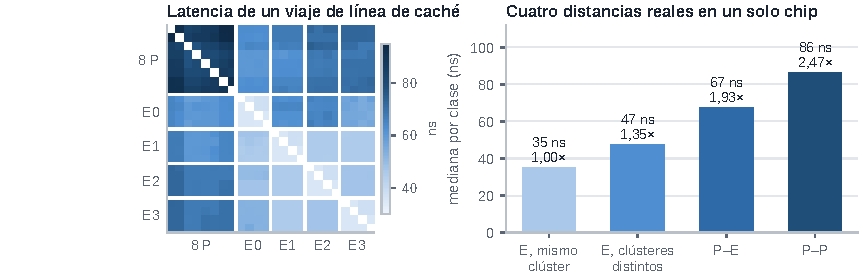
\includegraphics[width=0.62\linewidth]{topologia.pdf}
  \caption{Mapa de latencia caché-a-caché entre los 24 núcleos del Core Ultra 9 285 (\texttt{topologia/matriz\_nucleos.csv}). Cada casilla es una pareja de núcleos (más oscuro = viaje más lento). Los cuatro cuadros claros sobre la diagonal (CPUs 8--23) revelan los cuatro clústeres de núcleos E (35,0\,ns dentro frente a 47,4\,ns entre clústeres y 86,3\,ns entre núcleos P, CPUs 0--7).}
  \label{fig:topologia}
\end{figure}

% ==============================================================================
\section{Verificación de Corrección y Cota \emph{Wait-Free}}
% ==============================================================================

\subsection{Detectores automáticos (ASan, UBSan y TSan) y rotura de reglas}
Un algoritmo concurrente rápido no sirve de nada si corrompe memoria. Para comprobar la corrección se emplearon tres detectores automáticos del compilador (\emph{sanitizadores}):
\begin{itemize}
  \item \textbf{AddressSanitizer (ASan):} vigila cada lectura y escritura en memoria y detiene el programa al instante si alguien accede a memoria ya liberada (\emph{use-after-free}), libera dos veces (\emph{double-free}) o deja fugas de memoria.
  \item \textbf{ThreadSanitizer (TSan):} vigila accesos simultáneos de varios hilos a la misma dirección sin sincronización atómica (\emph{carreras de datos}). En Linux se invocó con \texttt{setarch -R}, que desactiva temporalmente la aleatorización de direcciones de memoria (ASLR) del kernel para evitar incompatibilidades con el mapa interno de TSan.
  \item \textbf{UndefinedBehaviorSanitizer (UBSan):} detecta operaciones inválidas en C++ como desbordamientos de enteros o alineaciones incorrectas.
\end{itemize}

Antes de fiarnos de un resultado de «0 errores», hay que demostrar que la alarma funciona de verdad. La Figura~\ref{fig:asan} muestra nuestra prueba de estrés (\texttt{codigo/estres\_asan.cpp}, con 10\,\% \texttt{store} y 90\,\% \texttt{load} sobre una única celda compartida): la versión ingenua en dos pasos dispara de inmediato un \emph{heap-use-after-free} (o \emph{double-free}), mientras que el código original de los autores~\cite{dewolff2024repo} completa millones de operaciones con \textbf{0 errores} tanto bajo ASan como bajo TSan. Además, auditamos a todos los rivales mediante \textbf{26 pruebas de sanitizadores} (\texttt{10\_sanitizers\_rivales.txt}): 12 con ASan+UBSan y 4 con TSan en \texttt{bench.cpp}, más 10 con ASan+UBSan sobre el \texttt{bench\_stack} oficial en Docker (incluyendo Folly y Anderson), todas con \textbf{0 avisos}, confirmando que ningún rival obtiene ventaja rompiendo la memoria.

\begin{figure}[H]
  \centering
  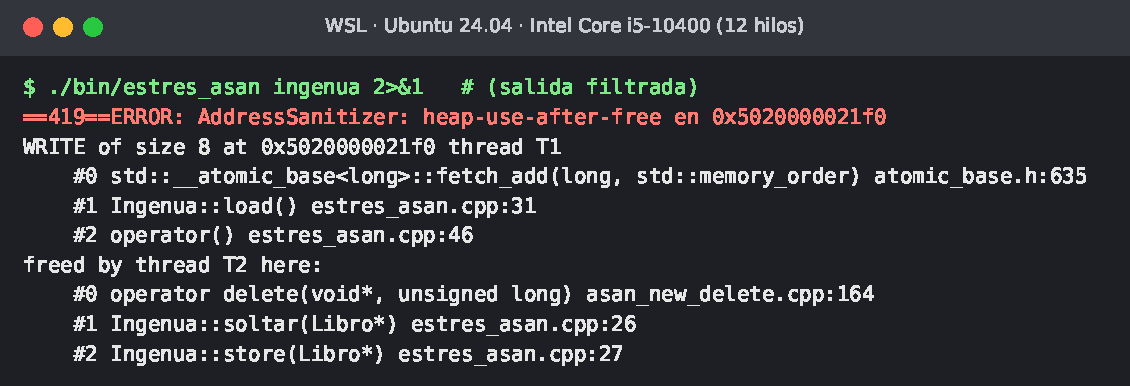
\includegraphics[width=0.90\linewidth,height=0.34\textheight,keepaspectratio]{captura_asan_ingenua.pdf}\\[4pt]
  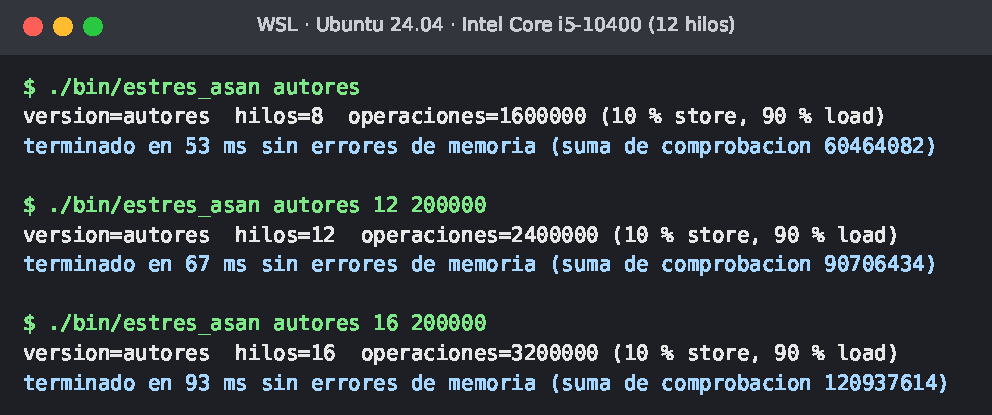
\includegraphics[width=0.72\linewidth,height=0.16\textheight,keepaspectratio]{captura_asan_autores.pdf}
  \caption{Verificación con AddressSanitizer (\texttt{estres\_asan.cpp}). Arriba: la lectura ingenua en dos pasos hace saltar al instante el detector por \emph{heap-use-after-free}. Abajo: la implementación de los autores completa 1,6\,M, 2,4\,M y 3,2\,M operaciones (8, 12 y 16 hilos) sin un solo error.}
  \label{fig:asan}
\end{figure}

Para comprobar que las reglas del paper no son adornos matemáticos sino requisitos imprescindibles, las rompimos a propósito en nuestro boceto didáctico en C++ ($P = 8, C = 16$, 8 hilos, 4 millones de operaciones) y en un simulador paso a paso de intercalados entre hilos (\texttt{simulador/buscar.js}, 20\,000 ejecuciones por variante). La Tabla~\ref{tab:correccion} muestra el resultado: al quitar la salida temprana («salir si otro hilo ya recargó»), el algoritmo sigue sin corromper memoria pero dispara hasta \textbf{45--55 reintentos de \texttt{CAS}} con $P = 8$, perdiendo su garantía \emph{wait-free}; y al violar la regla R-1 poniendo $C = P = 8$, aparecen decenas de miles de errores y fugas de memoria.

\begin{table}[H]
\centering
\caption{Pruebas de corrección, variantes rotas a propósito y simulador de intercalados en ambos equipos.}
\label{tab:correccion}
\small
\begin{tabularx}{\linewidth}{@{}l >{\raggedright\arraybackslash}X >{\raggedright\arraybackslash}X >{\raggedright\arraybackslash}X@{}}
\toprule
\textbf{Prueba / Variante} & \textbf{Qué evalúa} & \textbf{Core i5-10400 (WSL2)} & \textbf{Core Ultra 9 285} \\
\midrule
ASan + TSan (Autores, 8--16 hilos) & Ausencia de carreras y \emph{use-after-free} & \textbf{0 errores}, \textbf{0 avisos} & \textbf{0 errores}, \textbf{0 avisos} \\
Sanitizadores en los 5 rivales & Que ningún rival gane corrompiendo memoria & — & \textbf{26 pruebas, 0 avisos} \\
Boceto Paper ($P=8, C=16$, 4\,M ops) & Cota $\le P$ y contabilidad exacta de vales & \textbf{0 errores}, 0 fugas, máx.\ \textbf{8} CAS & \textbf{0 errores}, 0 fugas, máx.\ \textbf{6} CAS \\
Boceto sin salida temprana & Quitar salida cuando $w_{\text{nuevo}} > w_{\text{actual}}$ & 0 errores, pero \textbf{55 CAS} ($> P$) & 0 errores, pero \textbf{45 CAS} ($> P$) \\
Boceto $C = P = 8$ (viola R-1) & El taco no tiene el doble de vales que hilos & \textbf{63\,101 errores}, 3\,808 fugas & \textbf{42\,348 errores}, 4\,280 fugas \\
Simulador ($P=3, C=6$ y $P=4, C=8$) & Comprueba invariantes tras cada paso atómico & \textbf{0 fallos} en 1\,909\,884 pasos (máx.\ 4 CAS; 80,1\,\% en 1 intento). Variantes rotas: 4\,796 (\emph{UAF}, 6 pasos), 5\,089 ($w<0$, 2 pasos), 1\,171 (sin reserva, 6 pasos), 5\,467 (desborde, 7 pasos) & — \\
\bottomrule
\end{tabularx}
\end{table}

\subsection{Comprobación directa de la cota \emph{wait-free} en el código real}
Con los parámetros reales del código de los autores ($P = 65\,536$ hilos máximos y $C = 524\,287$ vales en el taco), casi nunca hace falta recargar porque un escritor suele cambiar la celda antes de que se consuman cientos de miles de vales. Para poner a prueba de verdad la promesa «la recarga reintenta como mucho $P$ veces», instrumentamos una copia del código real (\texttt{cota\_cas.cpp}) contando cada intento de \texttt{CAS}, primero con los valores reales y después encogiendo el talonario a $P = 32$ y $C = 64$ para forzar millones de recargas simultáneas (Figura~\ref{fig:cota_cas} y Tabla~\ref{tab:cota_cas}). En \textbf{64,4 millones de recargas forzadas} sumando las 18 configuraciones probadas, más del 84\,\% terminó al primer intento y el máximo absoluto fue de \textbf{8 intentos de \texttt{CAS}} (muy por debajo del tope teórico de 32), con 0 errores.

\begin{figure}[H]
  \centering
  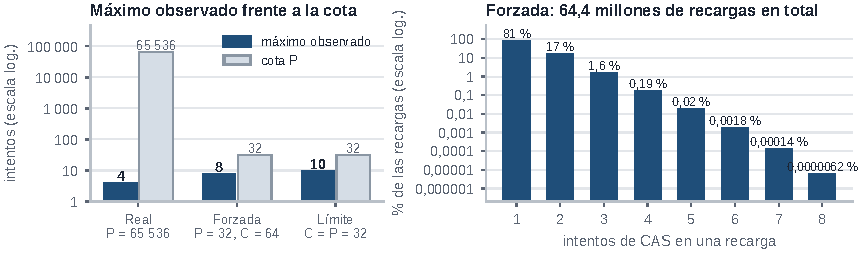
\includegraphics[width=0.76\linewidth]{cota_cas.pdf}
  \caption{Distribución y máximo de intentos de \texttt{CAS} por recarga en el código real de los autores instrumentado (\texttt{cota\_cas.csv}, Core Ultra 9 285). Incluso forzando millones de recargas con un taco pequeño ($P=32, C=64$), el máximo observado (8) queda muy por debajo de la cota teórica $P=32$.}
  \label{fig:cota_cas}
\end{figure}

\begin{table}[H]
\centering
\caption{Verificación de la cota \emph{wait-free} de intentos de \texttt{CAS} en el código real de los autores (\texttt{cota\_cas.csv}, Core Ultra 9 285).}
\label{tab:cota_cas}
\footnotesize
\setlength{\tabcolsep}{4pt}
\begin{tabularx}{\linewidth}{@{}l c r r r c >{\raggedright\arraybackslash}X@{}}
\toprule
\textbf{Variante} & \textbf{Hilos} & \textbf{Máx.\ recargas} & \textbf{Máx.\ CAS} & \textbf{Cota $P$} & \textbf{Err.} & \textbf{Distribución observada} \\
\midrule
Real ($P{=}65\,536, C{=}524\,287$) & 2--32 & 1\,158 (0\,\% \texttt{st.}) & \textbf{4} & 65\,536 & 0 & 80,2\,\% en 1 intento (24 h, 0\,\% \texttt{store}) \\
Forzada ($P{=}32, C{=}64$, R-1) & 2--32 & 8\,061\,142 (64,4\,M tot.) & \textbf{8} & 32 & 0 & 84,0\,\% en 1; 14,2\,\% en 2; solo 4/7,02\,M en 8 \\
Límite ($P{=}32, C{=}32$, sin R-1) & 8, 24 & 15\,600\,117 & 10 & 32 & 0$^*$ & Recarga casi siempre; rinde $\approx 0,5\times$ \\
\bottomrule
\end{tabularx}
\par\vspace{2pt}{\footnotesize $^*$Con $\text{hilos} \le P$ no llegó a desbordar en esta prueba, pero viola R-1 y degrada el rendimiento a la mitad.}
\end{table}

% ==============================================================================
\section{Rendimiento Concurrente y Controles Metodológicos (Figura 5)}
% ==============================================================================

\subsection{Comparación con los cinco algoritmos oficiales en el Core Ultra 9 285}
Para leer las gráficas de esta sección conviene recordar dos reglas sencillas. Primero, \textbf{no comparamos si un ordenador es más rápido que otro, sino el orden y la proporción entre algoritmos}: como nuestro Core Ultra 9 285 es mucho más reciente que los Xeon del paper, expresamos cada rival como múltiplo de Autores ($0,50\times$ significa «rinde la mitad que Autores»; $2,00\times$, «rinde el doble»). Segundo, en los paneles con una sola pila ($n=1$) \textbf{las curvas caen bruscamente al pasar de 1 a 3 hilos}: no es un error de medida, sino el efecto del «único cuaderno» explicado en la Sección~1.2 (con 1 hilo el dato nunca sale de su caché local; con 3 hilos la línea de caché empieza a rebotar entre núcleos). En cambio, en el último panel ($n=10^6$, un millón de pilas) los hilos casi nunca coinciden en la misma pila y las curvas suben al añadir hilos.

Las Figuras~\ref{fig:fig5_curvas} y~\ref{fig:fig5_relativo} muestran las curvas en los seis escenarios del paper y la proporción de cada rival respecto a Autores con toda la CPU llena (24 hilos aquí frente a 144 en el paper). La Tabla~\ref{tab:fig5_completa} recoge las medianas tanto dentro de Docker como fuera del contenedor.

\begin{figure}[H]
  \centering
  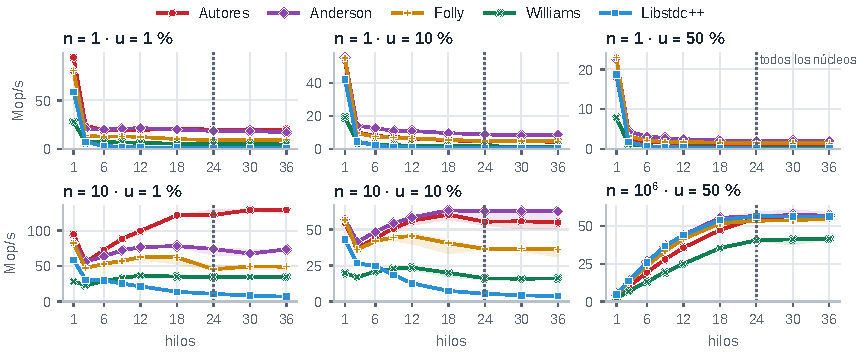
\includegraphics[width=0.94\linewidth]{fig5_docker.pdf}
  \caption{Rendimiento en millones de operaciones por segundo (Mop/s, mediana de 5 rondas y banda mín.--máx.) de los 5 algoritmos oficiales en el Core Ultra 9 285 con Docker. Cada recuadro cambia el número de pilas ($n$) y el porcentaje de escrituras ($u$). La raya vertical discontinua marca los 24 núcleos físicos (equivalente a los 144 hilos del paper).}
  \label{fig:fig5_curvas}
\end{figure}

\begin{figure}[H]
  \centering
  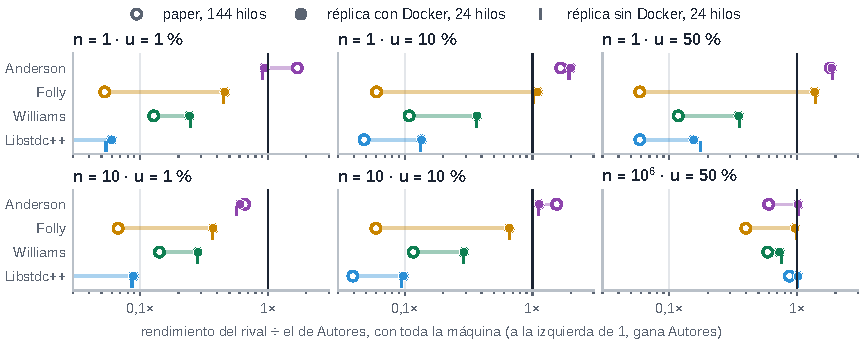
\includegraphics[width=0.90\linewidth]{relativo_paper_replica.pdf}
  \caption{Rendimiento relativo respecto a Autores ($1 = \text{empate}$; izquierda = gana Autores; derecha = gana el rival) con toda la CPU llena: círculos huecos para el paper (144 hilos) y rellenos para nuestra réplica en el Core Ultra 9 285 (24 hilos). Si el círculo hueco y el relleno caen juntos, la réplica coincide con el paper.}
  \label{fig:fig5_relativo}
\end{figure}

\begin{table}[H]
\centering
\caption{Rendimiento a máquina llena: Paper (144 hilos) frente a Réplica en Core Ultra 9 285 (24 hilos, con y sin Docker), en Mop/s y proporción respecto a Autores. $\tau$ es la correlación de orden de Kendall en Docker ($+1$ = mismo ranking exacto).}
\label{tab:fig5_completa}
\scriptsize
\setlength{\tabcolsep}{3.5pt}
\begin{tabular}{@{}l l r r r r r c@{}}
\toprule
\textbf{Escenario} & \textbf{Tanda} & \textbf{Autores} & \textbf{Anderson} & \textbf{Folly} & \textbf{Williams} & \textbf{Libstdc++} & $\boldsymbol{\tau}$ \\
\midrule
\multirow{3}{*}{$n=1,\ u=1\,\%$}
  & Paper (144 h) & 5,86 (1,00$\times$) & \textbf{9,98 (1,70$\times$)} & 0,31 (0,05$\times$) & 0,75 (0,13$\times$) & 0,11 (0,02$\times$) & \multirow{3}{*}{$+0,60$} \\
  & Docker (24 h) & \textbf{19,81 (1,00$\times$)} & 18,64 (0,94$\times$) & 9,11 (0,46$\times$) & 4,83 (0,24$\times$) & 1,19 (0,06$\times$) & \\
  & Nativo (24 h) & \textbf{19,90 (1,00$\times$)} & 18,11 (0,91$\times$) & 8,94 (0,45$\times$) & 4,96 (0,25$\times$) & 1,08 (0,05$\times$) & \\
\midrule
\multirow{3}{*}{$n=1,\ u=10\,\%$}
  & Paper (144 h) & 0,83 (1,00$\times$) & \textbf{1,38 (1,66$\times$)} & 0,05 (0,06$\times$) & 0,09 (0,11$\times$) & 0,04 (0,05$\times$) & \multirow{3}{*}{$+0,60$} \\
  & Docker (24 h) & 4,43 (1,00$\times$) & \textbf{8,81 (1,99$\times$)} & 4,84 (1,09$\times$) & 1,63 (0,37$\times$) & 0,60 (0,14$\times$) & \\
  & Nativo (24 h) & 4,54 (1,00$\times$) & \textbf{8,77 (1,93$\times$)} & 4,64 (1,02$\times$) & 1,65 (0,36$\times$) & 0,60 (0,13$\times$) & \\
\midrule
\multirow{3}{*}{$n=1,\ u=50\,\%$}
  & Paper (144 h) & 0,17 (1,00$\times$) & \textbf{0,31 (1,82$\times$)} & 0,01 (0,06$\times$) & 0,02 (0,12$\times$) & 0,01 (0,06$\times$) & \multirow{3}{*}{$+0,40$} \\
  & Docker (24 h) & 1,07 (1,00$\times$) & \textbf{2,00 (1,87$\times$)} & 1,47 (1,37$\times$) & 0,37 (0,35$\times$) & 0,17 (0,16$\times$) & \\
  & Nativo (24 h) & 1,07 (1,00$\times$) & \textbf{2,03 (1,90$\times$)} & 1,50 (1,40$\times$) & 0,38 (0,36$\times$) & 0,19 (0,17$\times$) & \\
\midrule
\multirow{3}{*}{$n=10,\ u=1\,\%$}
  & Paper (144 h) & \textbf{46,34 (1,00$\times$)} & 30,45 (0,66$\times$) & 3,12 (0,07$\times$) & 6,57 (0,14$\times$) & 1,09 (0,02$\times$) & \multirow{3}{*}{$+0,80$} \\
  & Docker (24 h) & \textbf{121,90 (1,00$\times$)} & 74,04 (0,61$\times$) & 45,51 (0,37$\times$) & 34,69 (0,28$\times$) & 10,82 (0,09$\times$) & \\
  & Nativo (24 h) & \textbf{126,70 (1,00$\times$)} & 72,31 (0,57$\times$) & 46,84 (0,37$\times$) & 35,55 (0,28$\times$) & 10,95 (0,09$\times$) & \\
\midrule
\multirow{3}{*}{$n=10,\ u=10\,\%$}
  & Paper (144 h) & 8,90 (1,00$\times$) & \textbf{13,75 (1,54$\times$)} & 0,53 (0,06$\times$) & 1,04 (0,12$\times$) & 0,35 (0,04$\times$) & \multirow{3}{*}{$+0,80$} \\
  & Docker (24 h) & 55,40 (1,00$\times$) & \textbf{62,67 (1,13$\times$)} & 36,55 (0,66$\times$) & 16,08 (0,29$\times$) & 5,42 (0,10$\times$) & \\
  & Nativo (24 h) & 55,67 (1,00$\times$) & \textbf{62,10 (1,12$\times$)} & 36,78 (0,66$\times$) & 16,09 (0,29$\times$) & 5,24 (0,09$\times$) & \\
\midrule
\multirow{3}{*}{$n=10^6,\ u=50\,\%$}
  & Paper (144 h) & \textbf{129,32 (1,00$\times$)} & 77,50 (0,60$\times$) & 51,41 (0,40$\times$) & 76,12 (0,59$\times$) & 112,68 (0,87$\times$) & \multirow{3}{*}{$+0,20$} \\
  & Docker (24 h) & 55,37 (1,00$\times$) & 56,50 (1,02$\times$) & 53,39 (0,96$\times$) & 40,39 (0,73$\times$) & 56,34 (1,02$\times$) & \\
  & Nativo (24 h) & 54,66 (1,00$\times$) & 56,21 (1,03$\times$) & 54,12 (0,99$\times$) & 41,28 (0,76$\times$) & 54,78 (1,00$\times$) & \\
\bottomrule
\end{tabular}
\end{table}

\textbf{Lo que se reproduce fielmente:}
\begin{enumerate}
  \item \textbf{Frente a Libstdc++ y Williams (afirmaciones 1 y 2):} Libstdc++ se hunde al aumentar la contención hasta rendir solo un $0,05\times$--$0,17\times$ de Autores (baja de $58,47$ a $1,19$\,Mop/s en $n=1, u=1\,\%$) porque su pestillo de 1 bit obliga a los hilos a esperar dando vueltas en cola. Williams queda por debajo de Autores en los seis escenarios ($0,24\times$--$0,76\times$) porque cada lectura paga el peaje de dos bucles de \texttt{DWCAS} de 16 bytes.
  \item \textbf{El equilibrio frente a Anderson (afirmaciones 4 y 6):} cuando casi todas las operaciones son lecturas repartidas en varias pilas ($n=10, u=1\,\%$), Autores brilla con $121,90$\,Mop/s frente a $74,04$\,Mop/s de Anderson ($+65\,\%$ en Docker y $+75\,\%$ sin Docker). Por el contrario, con muchas escrituras sobre una sola pila ($n=1, u \ge 10\,\%$), Anderson gana casi por el doble ($1,87\times$--$1,99\times$), exactamente por la razón de diseño que explica el paper: en Autores cada lectura escribe en la celda compartida (al restar un vale) y hace fallar los \texttt{CAS} de los escritores, mientras que en Anderson leer no modifica la celda. En $n=1, u=1\,\%$, en el paper Anderson solo adelantaba a Autores a partir de 54 hilos (a 18 y 36 hilos rendía $0,72\times$ y $0,89\times$); aquí, a 24 hilos, rinde $0,94\times$, coherente con la menor escala de hilos de nuestra CPU.
\end{enumerate}

\textbf{El misterio de Folly (afirmación 3, no reproducida):} en el paper, Folly aparece unas veinte veces por debajo de Autores bajo contención ($0,05\times$--$0,07\times$). En el Core Ultra 9 285 rinde mucho mejor (entre $0,37\times$ y $1,40\times$): Autores le gana en 3 escenarios, empatan en 2 ($n=1, u=10\,\%$ y $n=10^6$) y \textbf{Folly gana claramente en $n=1, u=50\,\%$} ($1,47$ frente a $1,07$\,Mop/s en Docker; $1,50$ frente a $1,07$ sin Docker). Podría pensarse que esto se debe a no tener 4 \emph{sockets}, pero la Figura~\ref{fig:un_hilo} y la Tabla~\ref{tab:folly_1hilo} descartan esa explicación: \textbf{la brecha ya existe con un solo hilo}, donde no hay competencia ni líneas de caché viajando entre núcleos, mientras que Williams con 1 hilo sí reproduce casi al milímetro las proporciones del paper.

\begin{figure}[H]
  \centering
  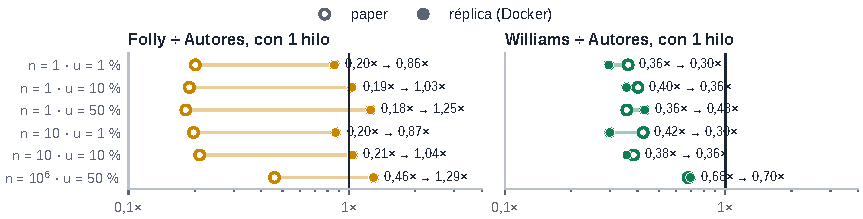
\includegraphics[width=0.78\linewidth]{un_hilo.pdf}
  \caption{Prueba clave sobre Folly con \textbf{un solo hilo}: la diferencia respecto al paper ya está presente sin concurrencia ($0,86\times$--$1,29\times$ aquí frente a $0,18\times$--$0,46\times$ en el paper), mientras que Williams sí coincide.}
  \label{fig:un_hilo}
\end{figure}

\begin{table}[H]
\centering
\caption{Rendimiento relativo a Autores con \textbf{un solo hilo} (\texttt{tablas.md}): Folly ya diverge del paper sin contención, mientras Williams coincide.}
\label{tab:folly_1hilo}
\footnotesize
\setlength{\tabcolsep}{5pt}
\begin{tabular}{@{}l c c c c c@{}}
\toprule
\textbf{Escenario (1 hilo)} & \textbf{Folly Paper} & \textbf{Folly Docker} & \textbf{Folly Nativo} & \textbf{Williams Paper} & \textbf{Williams Docker} \\
\midrule
$n = 1,\ u = 1\,\%$ & $0,20\times$ & $0,86\times$ & $0,88\times$ & $0,36\times$ & $0,30\times$ \\
$n = 1,\ u = 50\,\%$ & $0,18\times$ & $1,25\times$ & $1,25\times$ & $0,36\times$ & $0,43\times$ \\
$n = 10,\ u = 10\,\%$ & $0,21\times$ & $1,04\times$ & $1,04\times$ & $0,38\times$ & $0,36\times$ \\
$n = 10^6,\ u = 50\,\%$ & $0,46\times$ & $1,29\times$ & $1,24\times$ & $0,68\times$ & $0,70\times$ \\
\bottomrule
\end{tabular}
\end{table}

\subsection{Controles metodológicos: Docker, recorte temporal y compartición falsa}
\label{sec:controles_rend}
Para asegurarnos de que ninguna diferencia viniera de nuestras herramientas de medida, realizamos tres controles directos:

\paragraph{1. Docker no altera los binarios oficiales (Figura~\ref{fig:docker_y_alineado}a).}
Al compilar y ejecutar exactamente los mismos programas oficiales fuera de Docker (\texttt{nativo\_oficial/}), las medianas del cociente nativo/Docker en los 54 puntos de cada algoritmo fueron $1,00\times$ (Autores, Folly, Libstdc++), $0,99\times$ (Anderson) y $1,01\times$ (Williams). De los \textbf{270 puntos totales}, \textbf{259 cambian menos de un 10\,\%} y \textbf{236 menos de un 5\,\%}. Un control adicional alternando el mismo binario dentro y fuera dio mediana de $1,02\times$. Docker actúa como correr en la misma pista llevando un dorsal: no frena al programa.

\paragraph{2. Validación del recorte $2\,\text{s} \times 5$ frente a la receta larga $10\,\text{s} \times 7$.}
Al repetir los 6 escenarios a 24 hilos con la receta exacta del paper ($7 \times 10$\,s en un mismo proceso, fuera de Docker, \texttt{nativo\_oficial/paridad.csv}), la mitad de los 30 puntos se desvía menos de un $6,7\,\%$ (extremos de $-10,0\,\%$ en Libstdc++ $n=10^6$ a $+19,0\,\%$ en Folly $n=10, u=10\,\%$). El orden de los 5 algoritmos se conserva idéntico en 4 de los 6 escenarios, y en los otros 2 solo se intercambian algoritmos ya empatados ($<4\,\%$). Existe un pequeño sesgo sistemático (la versión corta en procesos nuevos rinde algo más en 23 de 25 puntos con contención y algo menos en los 5 puntos de $n=10^6$), por lo que este informe nunca interpreta márgenes pequeños como victorias.

\paragraph{3. Compartición falsa y desborde de caché L3 en \texttt{bench.cpp} (Figura~\ref{fig:docker_y_alineado}b y Tabla~\ref{tab:alineacion}).}
Al comparar nuestro banco independiente \texttt{codigo/bench.cpp} con el binario oficial en $n=10$, Autores rendía tres veces menos. El culpable resultó ser una sola línea de código: mientras el programa oficial separaba cada pila en memoria con \texttt{alignas(128)} (reservando 128 bytes para cada una), en \texttt{bench.cpp} cada pila de Autores ocupaba solo 8 bytes, de modo que las 10 pilas cabían seguidas en 80 bytes ($\approx 2$ líneas de caché de 64 bytes). Como 10 renglones en la misma hoja de papel, hilos que trabajaban en pilas distintas se arrebataban continuamente las mismas 2 líneas (\textbf{compartición falsa}).

Al añadir únicamente \texttt{alignas(128)} en una copia (\texttt{nativo\_alineado/}), Autores saltó \textbf{$3,40\times$} en $n=10, u=1\,\%$ ($35,35 \to 120,27$\,Mop/s, igualando al binario oficial) y \textbf{$3,28\times$} en $n=10, u=10\,\%$, mientras que en el control $n=1$ (donde solo hay una pila, sin vecinas) no cambió nada ($1,00\times$--$1,02\times$). Pero al mirar $n=10^6$ apareció el efecto contrario: separar cada pila \textbf{frenó un 24--27\,\%}. El motivo es el tamaño del «cajón» de la caché L3 (36\,MB): sin alinear, un millón de pilas de 8--16 bytes ocupa 8--16\,MB y cabe dentro de la L3; al meter cada pila en una «carpeta» de 128 bytes pasa a ocupar 128\,MB, desborda la L3 y obliga a ir a la RAM sumando 207--265 bytes por operación (\texttt{alinear\_memoria.py}). Como prueba definitiva, en $n=10^5$ las pilas alineadas ocupan 12,8\,MB (vuelven a caber en la L3) y la penalización desaparece ($1,00\times$).

Además, en \texttt{bench.cpp} apareció una curiosidad instructiva: en $n=1, u=50\,\%$ con 24 hilos, el simple \texttt{Mutex} supera a Autores ($1,86$ frente a $1,15$\,Mop/s; $1,99$ frente a $1,17$ alineado). Como el \texttt{Mutex} duerme a los hilos que esperan, menos núcleos se pelean por la línea de caché a la vez; pero a cambio pierde la garantía \emph{wait-free} y paga colas de latencia enormes al despertar hilos.

\begin{figure}[H]
  \centering
  \begin{minipage}[t]{0.48\linewidth}
    \centering
    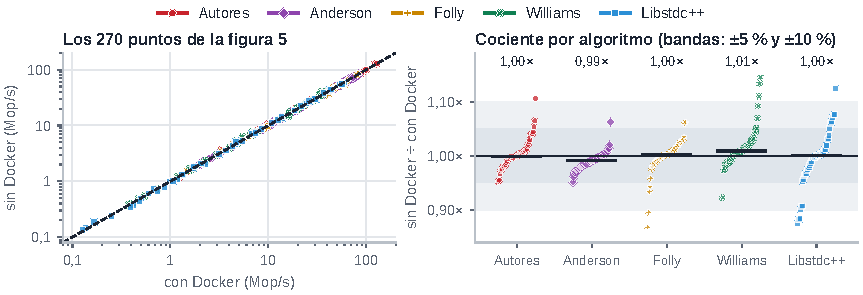
\includegraphics[width=\linewidth]{docker_frente_a_nativo.pdf}
    \par\vspace{2pt}{\footnotesize \textbf{(a)} Binarios oficiales: con Docker vs.\ sin Docker (259/270 puntos $<10\,\%$).}
  \end{minipage}\hfill
  \begin{minipage}[t]{0.48\linewidth}
    \centering
    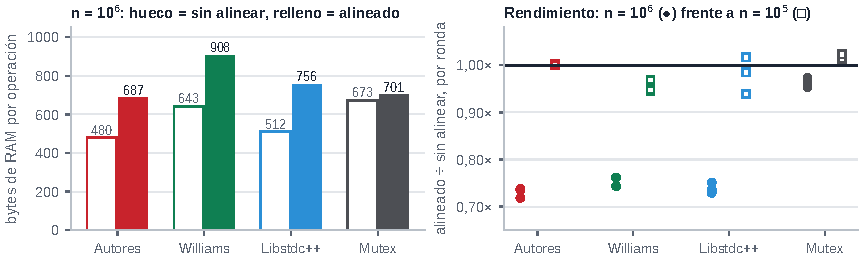
\includegraphics[width=\linewidth]{alineado_ram.pdf}
    \par\vspace{2pt}{\footnotesize \textbf{(b)} Efecto de \texttt{alignas(128)} en $n=10^5$ vs.\ $n=10^6$ (desborde de L3).}
  \end{minipage}
  \caption{Controles de validez interna en el Core Ultra 9 285.}
  \label{fig:docker_y_alineado}
\end{figure}

\begin{table}[H]
\centering
\caption{Efecto de \texttt{alignas(128)} en \texttt{bench.cpp} a 24 hilos (\texttt{tablas.md}: batería completa y tráfico real de RAM).}
\label{tab:alineacion}
\scriptsize
\setlength{\tabcolsep}{2.5pt}
\begin{tabular}{@{}l r r r r@{}}
\toprule
\textbf{Escenario (24 h)} & \textbf{Autores} & \textbf{Williams} & \textbf{Libstdc++} & \textbf{Mutex} \\
\midrule
$n{=}1$ (3 pan.): coc. & $1,00$--$1,02\times$ & $0,93$--$0,98\times$ & $0,92$--$1,01\times$ & $1,04$--$1,07\times$ \\
$n{=}10, u{=}1\,\%$ & $35,4 \to \mathbf{120,3}$ ($\mathbf{3,40\times}$) & $11,4 \to 28,8$ ($2,54\times$) & $6,7 \to 8,1$ ($1,20\times$) & $18,8 \to 25,2$ ($1,34\times$) \\
$n{=}10, u{=}10\,\%$ & $18,4 \to \mathbf{60,2}$ ($\mathbf{3,28\times}$) & $5,8 \to 8,5$ ($1,46\times$) & $3,6 \to 3,6$ ($1,02\times$) & $14,0 \to 20,4$ ($1,45\times$) \\
$n{=}10^6, u{=}50\,\%$ & $78,8 \to 57,6$ ($0,73\times$) & $50,7 \to 38,5$ ($0,76\times$) & $82,5 \to 60,9$ ($0,74\times$) & $66,6 \to 64,5$ ($0,97\times$) \\
$n{=}10^6$: RAM/op & $480 \to \mathbf{687}$ ($+207$\,B) & $643 \to \mathbf{908}$ ($+265$\,B) & $512 \to \mathbf{756}$ ($+244$\,B) & $673 \to 701$ ($+28$\,B) \\
\bottomrule
\end{tabular}
\end{table}

\subsection{Efecto de la distancia física entre clústeres de núcleos}
En el experimento de \textbf{dosis-respuesta} (subir gradualmente la distancia física manteniendo fijos los 4 hilos, Figura~\ref{fig:afinidad}), alejar los 4 hilos desde un mismo clúster E (35,0\,ns, compartiendo caché L2) hasta 4 clústeres distintos (47,4\,ns) reduce el rendimiento de Autores entre un \textbf{32\,\% y un 54\,\%} en los 5 escenarios con contención. En cambio, en el panel sin contención ($n=10^6$, que sirve de control del experimento), todos los algoritmos se mueven apenas $\pm 2\,\%$ (hasta $+3\,\%$ sin Docker): si los hilos no comparten cuaderno, la distancia no importa.

Al medir 14 parejas de 2 hilos en $n=1, u=50\,\%$, Autores cae un \textbf{44--45\,\%} justo al salir de la caché L2 compartida ($6,21 \to 3,41$\,Mop/s), pero prácticamente no cae más al pasar a núcleos P separados por 86,3\,ns ($3,29$\,Mop/s). Es un \textbf{efecto escalón}, no una rampa gradual: en cuanto dos hilos dejan de compartir la misma mesa (caché L2), da casi igual si la línea de caché viaja a la sala de al lado o al fondo del pasillo. Por su parte, Williams mostró en el binario oficial \texttt{bench\_stack} un hundimiento severo entre clústeres E ($-97\,\%$ en Docker: $3,05 \to 0,09$\,Mop/s; $-76\,\%$ sin Docker: $2,93 \to 0,70$\,Mop/s) que se repitió en los 7 pares distintos probados y no ocurre en \texttt{bench.cpp} ni al cambiar \texttt{std::atomic} por \texttt{boost::atomic}, apuntando al bucle muy apretado con \texttt{compare\_exchange\_weak} (una variante de \texttt{CAS} que puede fallar con facilidad cuando dos hilos se pisan en ritmo) del programa oficial.

\begin{figure}[H]
  \centering
  \begin{minipage}[t]{0.55\linewidth}
    \centering
    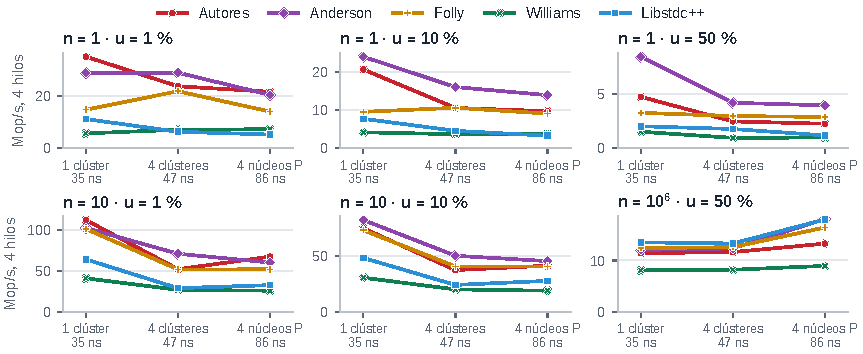
\includegraphics[width=\linewidth]{dosis_respuesta.pdf}
  \end{minipage}\hfill
  \begin{minipage}[t]{0.43\linewidth}
    \centering
    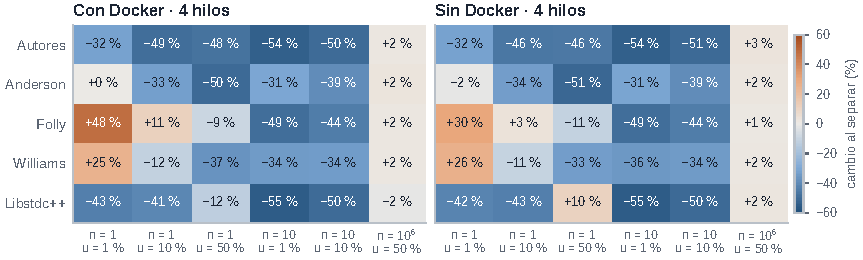
\includegraphics[width=\linewidth]{mapa_4hilos.pdf}
  \end{minipage}
  \caption{Simulación de distancia con 4 hilos en el Core Ultra 9 285. Izquierda: evolución al pasar de 1 clúster E (35\,ns) a 4 clústeres E (47\,ns) y 4 núcleos P (86\,ns). Derecha: cambio porcentual al separar 4 hilos entre clústeres E (azul = pierde al separar); el panel $n=10^6$ actúa como control plano ($\pm 2\,\%$).}
  \label{fig:afinidad}
\end{figure}

% ==============================================================================
\section{Latencia, Colas Extremas y el Candado Oculto de Williams (Figura 6)}
% ==============================================================================

La Figura~\ref{fig:fig6} muestra los \textbf{diagramas de caja} (\emph{boxplots}) de latencia obtenidos fuera de Docker con 15 rondas por punto (\texttt{nativo\_oficial\_fig6.png}). En cada caja, la raya central marca la \textbf{mediana (\texttt{p50})}, el rectángulo agrupa la mitad central de las medidas y los bigotes muestran los extremos más rápidos y más lentos. La fila superior corresponde a $p=1$ (un solo hilo sin competencia, escala lineal) y la inferior a $p=24$ (toda la CPU escribiendo a la vez, en \textbf{escala logarítmica}, donde cada escalón multiplica el tiempo por 10). La Figura~\ref{fig:candado_colas} detalla el hallazgo del candado oculto de Williams y las colas extremas (\texttt{p99,95}), y la Tabla~\ref{tab:latencia} resume todas las medianas frente al paper (incluyendo el valor correcto de \textbf{99,7\us{}} = 99\,700\,ns de Libstdc++ en \texttt{load}, $p=56$).

\begin{figure}[H]
  \centering
  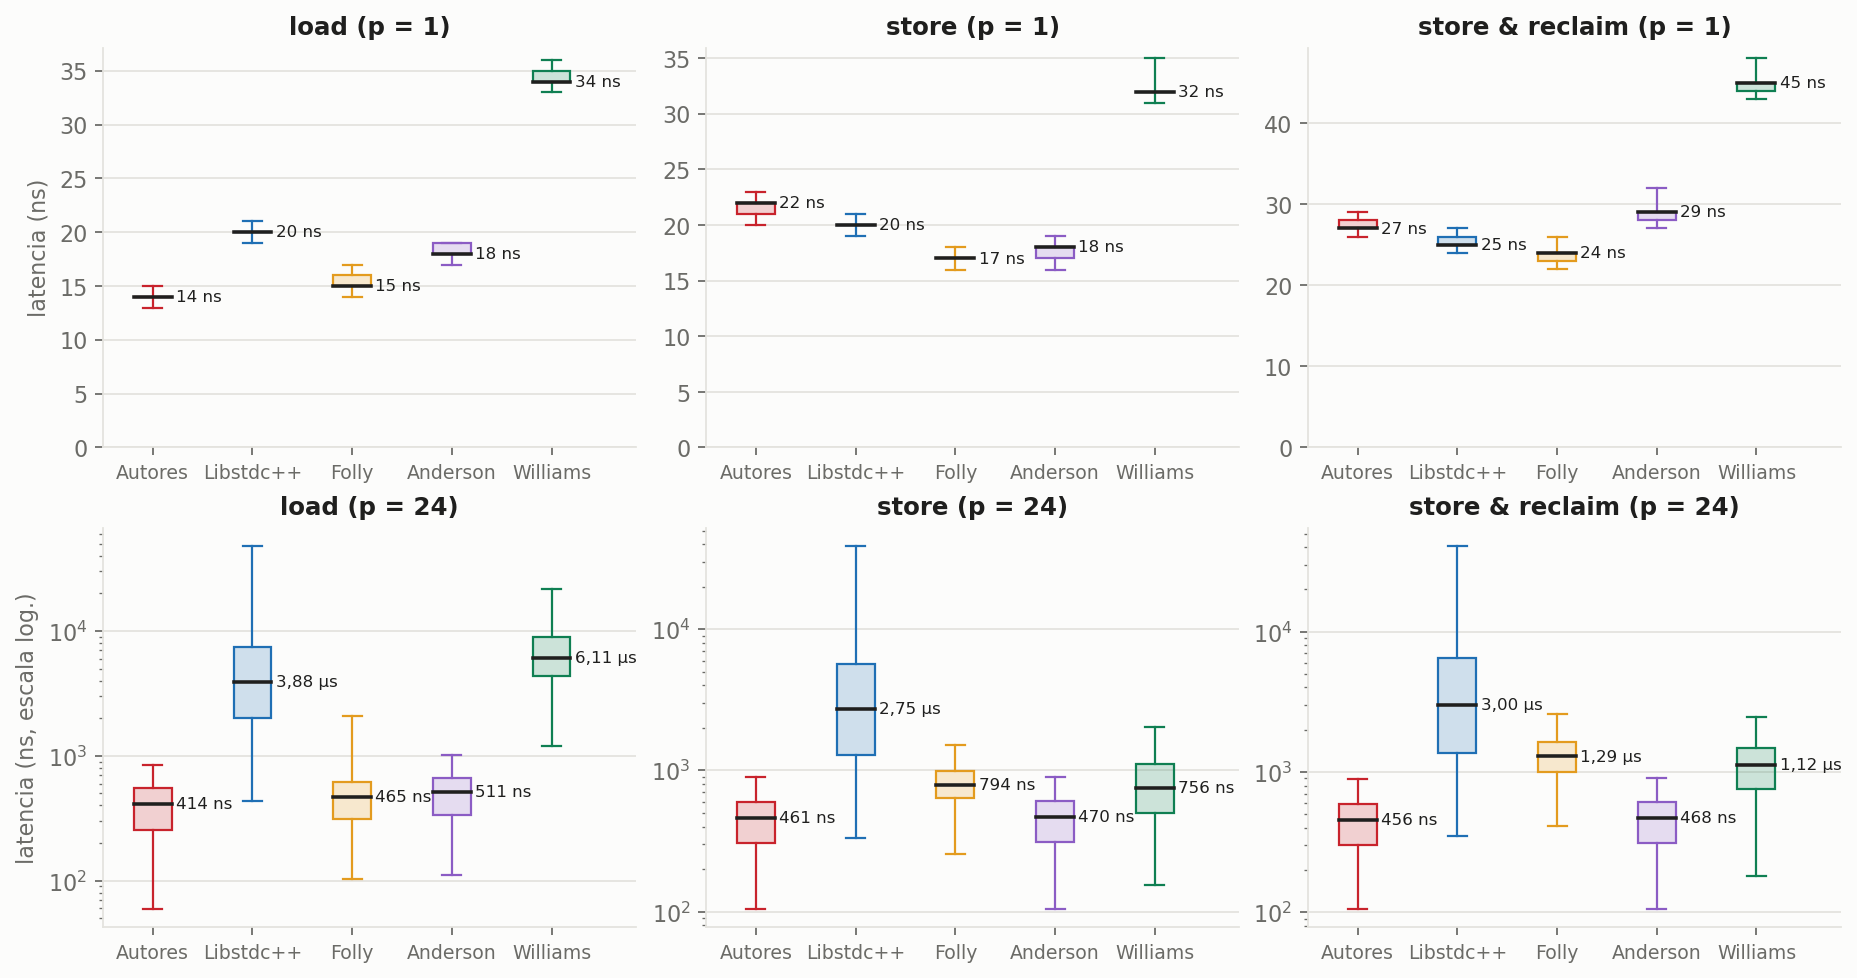
\includegraphics[width=0.90\linewidth]{nativo_oficial_fig6.png}
  \caption{Latencia de \texttt{load} (leer), \texttt{store} (escribir sin destruir) y \texttt{store \& reclaim} (escribir y liberar memoria) con los binarios oficiales sin Docker (15 rondas en el Core Ultra 9 285; Williams compilado con \texttt{-mcx16}). Arriba: sin contención ($p=1$). Abajo: 24 hilos a la vez ($p=24$, escala logarítmica).}
  \label{fig:fig6}
\end{figure}

\begin{figure}[H]
  \centering
  \begin{minipage}[t]{0.46\linewidth}
    \centering
    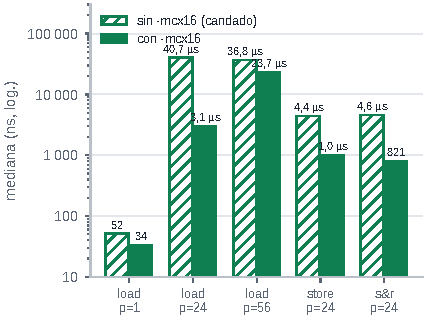
\includegraphics[width=\linewidth]{williams_candado.pdf}
    \par\vspace{2pt}{\footnotesize \textbf{(a)} Efecto de omitir \texttt{-mcx16} en Williams (\texttt{lock\_pool} frente a \texttt{cmpxchg16b}).}
  \end{minipage}\hfill
  \begin{minipage}[t]{0.50\linewidth}
    \centering
    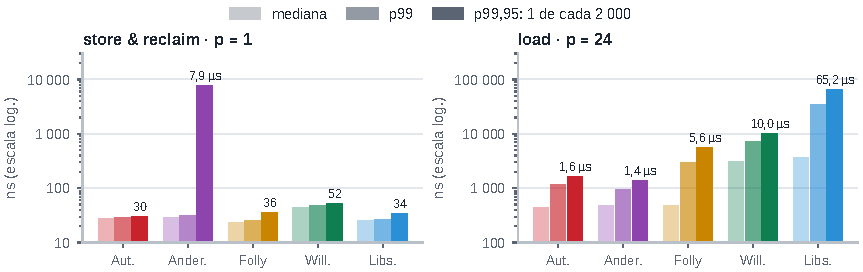
\includegraphics[width=\linewidth]{colas.pdf}
    \par\vspace{2pt}{\footnotesize \textbf{(b)} Colas \texttt{p50 / p99 / p99,95}: salto de Anderson cada 2\,000 retiradas.}
  \end{minipage}
  \caption{Auditoría de latencia: corrección del binario de Williams y comportamiento en los peores casos (colas).}
  \label{fig:candado_colas}
\end{figure}

\begin{table}[H]
\centering
\caption{Latencia con los binarios oficiales en el Core Ultra 9 285: medianas (\texttt{p50}) frente al paper y colas (\texttt{p99 / p99,95} en la tanda nativa de 15 rondas), en nanosegundos (menos es mejor).}
\label{tab:latencia}
\scriptsize
\setlength{\tabcolsep}{3.5pt}
\begin{tabular}{@{}l l r r r r r@{}}
\toprule
\textbf{Operación} & \textbf{Corte / Métrica} & \textbf{Autores} & \textbf{Anderson} & \textbf{Folly} & \textbf{Williams} & \textbf{Libstdc++} \\
\midrule
\multirow{5}{*}{\texttt{load}}
  & Paper $p{=}1$ (\texttt{p50}) & \textbf{23} & 28 & 24 & — & 29 \\
  & U9 Dock./Nat.\ $p{=}1$ (\texttt{p50}) & \textbf{14 / 14} & 18 / 18 & 15 / 15 & 34 / 34 & 20 / 20 \\
  & Paper $p{=}56$ (\texttt{p50}) & \textbf{1\,140} & 2\,580 & 11\,600 & — & 99\,700 \\
  & U9 Dock./Nat.\ $p{=}24$ (\texttt{p50}) & \textbf{437 / 414} & 488 / 511 & 473 / 465 & 3\,104 / 6\,106 & 3\,716 / 3\,882 \\
  & U9 Nat.\ $p{=}24$ (\texttt{p99 / 99,95}) & \textbf{848 / 1\,112} & 1\,014 / 1\,823 & 2\,091 / 4\,006 & 21\,670 / 32\,822 & 48\,062 / 90\,014 \\
\midrule
\multirow{4}{*}{\texttt{store}}
  & Paper $p{=}1$ (\texttt{p50}) & 33 & \textbf{28} & 37 & — & 36 \\
  & U9 Dock./Nat.\ $p{=}1$ (\texttt{p50}) & 22 / 22 & 18 / 18 & \textbf{17 / 17} & 32 / 32 & 20 / 20 \\
  & Paper $p{=}56$ (\texttt{p50}) & \textbf{1\,470} & 2\,840 & 2\,620 & — & 111\,000 \\
  & U9 Dock./Nat.\ $p{=}24$ (\texttt{p50}) & 507 / \textbf{461} & \textbf{483} / 470 & 832 / 794 & 1\,021 / 756 & 3\,411 / 2\,746 \\
\midrule
\multirow{5}{*}{\texttt{s\&r}}
  & Paper $p{=}1$ (\texttt{p50}) & 44 & 44 & 49 & — & \textbf{41} \\
  & U9 Dock./Nat.\ $p{=}1$ (\texttt{p50}) & 28 / 27 & 29 / 29 & \textbf{23 / 24} & 44 / 45 & 25 / 25 \\
  & U9 Nat.\ $p{=}1$ (\texttt{p99 / 99,95}) & 29 / \textbf{30} & 32 / \textbf{7\,740} & 26 / 31 & 48 / 51 & 27 / 38 \\
  & Paper $p{=}56$ (\texttt{p50}) & 1\,570 & \textbf{1\,250} & 5\,060 & — & 59\,300 \\
  & U9 Dock./Nat.\ $p{=}24$ (\texttt{p50}) & \textbf{462 / 456} & 470 / 468 & 1\,521 / 1\,290 & 821 / 1\,116 & 3\,248 / 3\,002 \\
\bottomrule
\end{tabular}
\par\vspace{2pt}{\footnotesize \texttt{s\&r} = \texttt{store \& reclaim} (guardar y liberar). Con $p=56$ en el paper y $p=24$ en el Core Ultra 9 285 toda la CPU física está ocupada.}
\end{table}

\textbf{Cuatro hallazgos clave en latencia:}
\begin{itemize}
  \item \textbf{El candado escondido de Williams (\texttt{-mcx16}):} el archivo \texttt{CMakeLists.txt} oficial del banco de latencia no incluía la bandera \texttt{-mcx16} (porque Williams estaba comentado en el artefacto). Al reactivarlo sin esa opción, la biblioteca \texttt{boost::\allowbreak atomic} de 16 bytes recurrió silenciosamente a una tabla interna de candados (\texttt{lock\_\allowbreak pool}) en lugar de usar la instrucción hardware \texttt{cmpxchg16b}, como cronometrar a un corredor con una mochila de piedras sin saberlo: el \texttt{load} a $p=24$ se disparó de \textbf{3\,104\,ns a 40\,680\,ns} ($13\times$). Recompilado con \texttt{-mcx16} (verificado en ensamblador con instrucciones \texttt{cmpxchg16b} y 0 llamadas al candado), Williams es el más lento con $p=1$, pero con contención \textbf{supera a Libstdc++} en 5--6 de los 6 cortes y a Folly en \texttt{store} y \texttt{store \& reclaim} con $p=24$ (afirmación 12: \emph{en parte}).
  \item \textbf{El pico periódico de Anderson en \texttt{p99,95}:} sin contención ($p=1$), en \texttt{store \& reclaim} Anderson va igual de rápido que los demás hasta \texttt{p99} (32\,ns), pero salta de golpe a \textbf{7\,740\,ns} sin Docker (\textbf{7\,895\,ns} en Docker) justo en el percentil 99,95 ($0,05\,\% = 1 \text{ de cada } 2\,000$ operaciones). Es la huella exacta del barrido de \emph{hazard pointers} que ParlayLib ejecuta cada 2\,000 objetos retirados.
  \item \textbf{Lo que significa \emph{wait-free} frente a \emph{lock-free} en la cola:} con 23 escritores cambiando la celda sin descanso ($p=24$), el lector de Autores termina en \textbf{1\,112\,ns} en \texttt{p99,95}, mientras que el lector \emph{lock-free} de Williams (que pierde repetidamente sus dos bucles de \texttt{DWCAS}) se dispara a \textbf{32\,822\,ns} y el \emph{spinlock} de Libstdc++ a \textbf{90\,014\,ns}.
  \item \textbf{Ruido entre rondas bajo contención:} mientras que con $p=1$ todas las rondas salen prácticamente idénticas (razón máx./mín.\ de $1,00\times$), con $p=24$ sin núcleos aislados la razón típica entre la ronda más lenta y la más rápida es de $3,40\times$ (5 rondas) y $5,75\times$ (15 rondas; como tirar un dado más veces, amplía el extremo entre el mejor y el peor intento pero estabiliza la mediana). Al subir a 15 rondas sin Docker, la supuesta mejora de \texttt{store \& reclaim} sobre \texttt{store} con contención (afirmación 11) se encogió a un 1--4\,\% ($461 \to 456$\,ns en $p=24$; $1\,531 \to 1\,480$\,ns en $p=56$), dentro del ruido, quedando en \emph{no se confirma}.
\end{itemize}

% ==============================================================================
\section{Memoria, Techo de RAM y Segundo Equipo (Core i5-10400)}
% ==============================================================================

\subsection{Memoria retenida y ancho de banda real de la controladora de memoria}
Con nuestra prueba \texttt{bench\_basura.cpp} (Figura~\ref{fig:memoria}a), donde la mitad de los hilos escribe y la otra mitad lee sin parar mientras contamos bloques vivos, se comprobó que los cinco algoritmos destruyen el \textbf{objeto de datos del usuario} en el acto (pico de 13--18 objetos vivos con 24 hilos, siempre por debajo del límite teórico de 37). Sin embargo, \textbf{Anderson retiene hasta 19\,960 bloques de control} en su caja de pendientes en Docker (\textbf{469\,KB}) y \textbf{20\,256 bloques} sin Docker (\textbf{476\,KB}), frente a 52--59 bloques ($\le 122$, unos 2,3--3,3\,KB y cero diferidos) en Autores, Folly, Williams y Libstdc++. Conviene añadir un matiz justo: menos de medio megabyte es un coste modesto, por lo que al mirar la memoria física total ocupada por el proceso (\textbf{RSS}, \emph{Resident Set Size}) en el escenario masivo $n=10^6$, la cifra la dominan los millones de nodos vivos y no la basura retenida: 1\,074\,MB (Autores), 1\,055\,MB (Folly y Libstdc++), 910\,MB (Anderson) y 1\,667\,MB (Williams).

Por otro lado, para comprobar si el cuádruple empate en $n=10^6$ (53--57\,Mop/s) se debe al único módulo DDR5 del Core Ultra 9, leímos los contadores físicos de la \textbf{controladora integrada de memoria (IMC)} (\texttt{medir\_memoria.py}, Figura~\ref{fig:memoria}b), que actúan como un cuentakilómetros en la única carretera hacia la RAM. Midieron un techo real en este único canal de \textbf{42,7\,GB/s leyendo en orden} y \textbf{36,8\,GB/s en lecturas al azar} (como saltar a páginas aleatorias de un libro, que es como acceden un millón de pilas). Con 24 hilos y $n=10^6$, Anderson (34,2\,GB/s), Libstdc++ (34,1\,GB/s) y Folly (32,8\,GB/s) alcanzan el \textbf{89--93\,\% de ese techo aleatorio}, lo que refuerza que la carretera de la RAM está casi saturada. Aun así, Autores mueve menos bytes por operación (515\,B y 27,8\,GB/s = 75\,\% del techo), por lo que demostrar definitivamente el límite de RAM requeriría instalar un segundo módulo de memoria.

\begin{figure}[H]
  \centering
  \begin{minipage}[t]{0.48\linewidth}
    \centering
    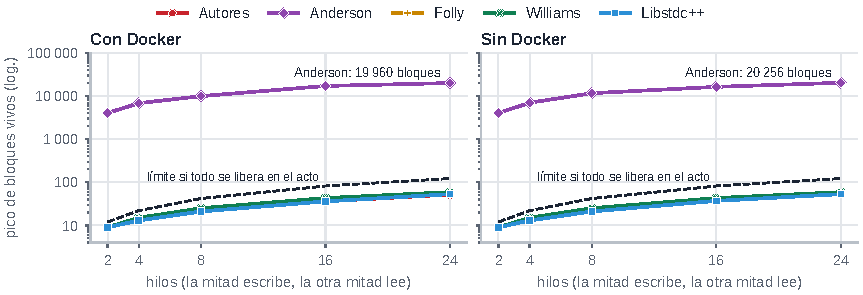
\includegraphics[width=\linewidth]{memoria_retenida.pdf}
    \par\vspace{2pt}{\footnotesize \textbf{(a)} Pico de bloques de control vivos (\texttt{bench\_basura}).}
  \end{minipage}\hfill
  \begin{minipage}[t]{0.48\linewidth}
    \centering
    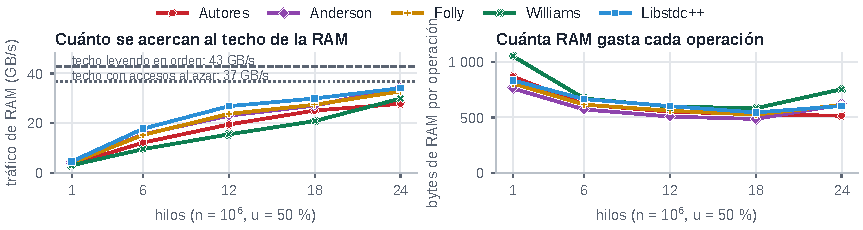
\includegraphics[width=\linewidth]{memoria_ram.pdf}
    \par\vspace{2pt}{\footnotesize \textbf{(b)} Tráfico real de RAM en $n=10^6$ frente al techo de 36,8\,GB/s.}
  \end{minipage}
  \caption{Consumo de memoria diferida (afirmación 13) y saturación del único canal de RAM en $n=10^6$ (afirmación 5).}
  \label{fig:memoria}
\end{figure}

\subsection{Segundo equipo: Intel Core i5-10400 frente a Intel Core Ultra 9 285}
Para comprobar si las conclusiones dependen de un procesador concreto, repetimos el banco propio (\texttt{codigo/ejecutar\_pruebas.sh}, \texttt{bench.cpp} sin alinear, \texttt{g++ 13.3}) en un segundo ordenador muy distinto: un \textbf{Intel Core i5-10400} de 6 núcleos y 12 hilos con SMT, 24\,GB DDR4 en doble canal y WSL2 Ubuntu 24.04. Las Figuras~\ref{fig:maquinas_comp} y~\ref{fig:maquinas_lat} y la Tabla~\ref{tab:dos_equipos} comparan directamente ambas máquinas ejecutando exactamente el mismo binario.

\begin{figure}[H]
  \centering
  \begin{minipage}[t]{0.48\linewidth}
    \centering
    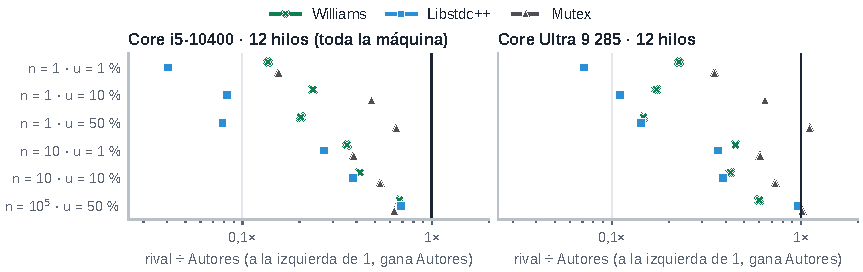
\includegraphics[width=\linewidth]{maquinas_orden.pdf}
    \par\vspace{2pt}{\footnotesize \textbf{(a)} Orden relativo a 12 hilos: Autores supera a Williams y Libstdc++ en ambas máquinas.}
  \end{minipage}\hfill
  \begin{minipage}[t]{0.48\linewidth}
    \centering
    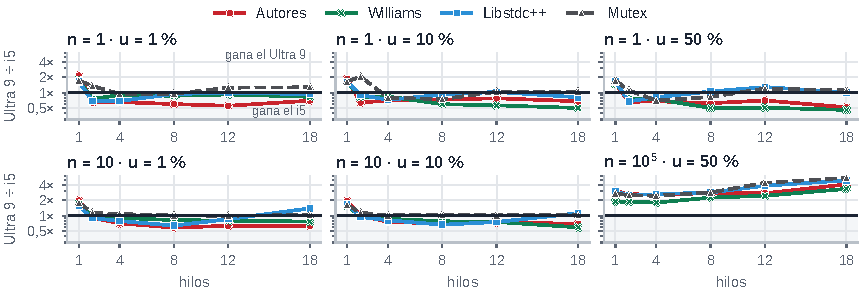
\includegraphics[width=\linewidth]{maquinas_cociente.pdf}
    \par\vspace{2pt}{\footnotesize \textbf{(b)} Cociente Ultra 9 $\div$ i5: gana Ultra 9 a 1 hilo y en $n=10^5$, pero pierde bajo contención.}
  \end{minipage}
  \caption{Comparativa directa Core Ultra 9 285 frente a Core i5-10400 ejecutando \texttt{codigo/bench.cpp}.}
  \label{fig:maquinas_comp}
\end{figure}

\begin{figure}[H]
  \centering
  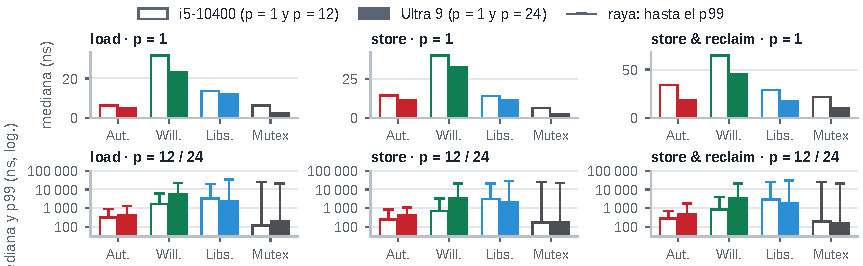
\includegraphics[width=0.80\linewidth]{maquinas_latencia.pdf}
  \caption{Latencia con \texttt{bench.cpp} en ambos equipos ($p=1$ y CPU llena: $p=12$ en i5, $p=24$ en Ultra 9). Aunque el \texttt{Mutex} aparenta menor mediana porque duerme a los hilos en espera, Autores conserva la cola \texttt{p99} más corta en las dos máquinas ($0,93\us{}$ en i5 y $1,32\us{}$ en Ultra 9 frente a $21$--$26\us{}$ del Mutex).}
  \label{fig:maquinas_lat}
\end{figure}

\begin{table}[H]
\centering
\caption{Comparación directa entre el Core i5-10400 y el Core Ultra 9 285 ejecutando el mismo binario (\texttt{bench.cpp}, 1\,s por punto; fuentes: \texttt{capturas/rendimiento.csv} y \texttt{david-ultra9-285/correccion/rendimiento.csv}), en Mop/s.}
\label{tab:dos_equipos}
\footnotesize
\setlength{\tabcolsep}{4pt}
\begin{tabular}{@{}l l r r c r r c@{}}
\toprule
\textbf{Escenario} & \textbf{Algoritmo} & \textbf{i5 (1\,h)} & \textbf{U9 (1\,h)} & \textbf{U9/i5} & \textbf{i5 (12\,h)} & \textbf{U9 (12\,h)} & \textbf{U9/i5} \\
\midrule
\multirow{4}{*}{$n=1,\ u=1\,\%$}
  & \textbf{Autores} & 44,83 & \textbf{96,94} & $\mathbf{2,16\times}$ & \textbf{39,13} & 21,79 & $\mathbf{0,56\times}$ \\
  & Williams & 19,48 & 34,83 & $1,79\times$ & 5,34 & 4,94 & $0,93\times$ \\
  & Libstdc++ & 33,53 & 55,65 & $1,66\times$ & 1,58 & 1,56 & $0,99\times$ \\
  & Mutex & 27,72 & 47,89 & $1,73\times$ & 6,07 & 7,61 & $1,25\times$ \\
\midrule
$n=1,\ u=50\,\%$ & \textbf{Autores} & 14,56 & \textbf{21,95} & $1,51\times$ & \textbf{2,32} & 1,64 & $0,71\times$ \\
$n=10,\ u=1\,\%$ (sin alinear) & \textbf{Autores} & 48,38 & \textbf{95,49} & $1,97\times$ & \textbf{50,61} & 32,20 & $0,64\times$ \\
$n=10^5,\ u=50\,\%$ & \textbf{Autores} & 4,67 & \textbf{14,31} & $\mathbf{3,07\times}$ & 26,69 & \textbf{73,23} & $\mathbf{2,74\times}$ \\
\bottomrule
\end{tabular}
\end{table}

El segundo equipo confirma todas las tendencias entre algoritmos: a 12 hilos en $n=1, u=1\,\%$, Autores rinde $7,3\times$ más que Williams y $24,8\times$ más que Libstdc++, y conserva la cola \texttt{p99} más corta en ambas máquinas (mientras la mediana baja del \texttt{Mutex} engaña porque la mayoría de hilos están dormidos, disparando su cola \texttt{p99} a 21--26\us{}). Además, deja una lección muy ilustrativa sobre arquitectura de procesadores: cuando los hilos trabajan sin estorbarse (1 hilo o $n=10^5$), el moderno Core Ultra 9 supera ampliamente al i5-10400 ($2,16\times$--$3,07\times$). En cambio, \textbf{bajo máxima contención ($n=1, u=1\,\%$, 12 hilos), el Core i5-10400 rinde casi el doble que el Core Ultra 9} ($39,13$ frente a $21,79$\,Mop/s). La hipótesis más verosímil —coherente con nuestra Sección~4.3, aunque pendiente de medir directamente fijando hilos en el i5— es que los 6 núcleos iguales en anillo del i5, con parejas de hilos SMT compartiendo literalmente la misma caché L1 y L2, se pasan la única línea caliente mucho más rápido que los clústeres híbridos P y E del Ultra 9 (47--86\,ns).

% ==============================================================================
\section{Veredicto Global, Limitaciones y Reproducibilidad}
% ==============================================================================

\subsection{Tabla maestra de las 15 afirmaciones del paper}
La Tabla~\ref{tab:veredicto} contrasta una por una las 15 afirmaciones experimentales del artículo usando cuatro etiquetas: \textbf{Se reproduce} (el dato medido confirma la afirmación), \textbf{En parte} (se cumple solo en ciertos cortes o con empate técnico), \textbf{No se reproduce} (nuestro hardware muestra lo contrario) y \textbf{No se confirma} (el efecto queda dentro del ruido entre rondas). El balance final es: \textbf{9 se reproducen · 2 en parte · 3 no se reproducen · 1 no se confirma}.

\begin{table}[H]
\centering
\caption{Veredicto experimental sobre las 15 afirmaciones del artículo de Euro-Par 2024~\cite{dewolff2024waitfree}.}
\label{tab:veredicto}
\footnotesize
\begin{tabularx}{\linewidth}{@{}r >{\raggedright\arraybackslash}p{4.6cm} >{\raggedright\arraybackslash}X l@{}}
\toprule
\textbf{\#} & \textbf{Afirmación del paper} & \textbf{Evidencia medida en la réplica} & \textbf{Veredicto} \\
\midrule
1 & Mucho más rápido que Libstdc++ & Gana con contención ($0,05\times$--$0,17\times$ en Ultra 9; $0,04\times$ en i5); empata en $n=10^6$ & \si \\
2 & Mucho más rápido que Williams & Gana en los 6 escenarios ($0,24\times$--$0,76\times$ en Ultra 9; $0,14\times$ en $n=1,u=1\,\%$ en i5) & \si \\
3 & Mucho más rápido que Folly & Gana 3, empata 2 y pierde 1 ($n=1,u=50\,\%$: $1,07$ vs.\ $1,47$\,Mop/s); brecha ya a 1 hilo & \no \\
4 & Con $u$ pequeño supera a Anderson & $+6\,\%$ en $n=1$ y $+65\,\%$ en $n=10$ con Docker ($+10\,\%$ y $+75\,\%$ sin Docker) & \si \\
5 & Con $n=10^6$ supera a Anderson & Pierde hasta 18 hilos y empata a $\approx 55$\,Mop/s desde 24 hilos (RAM 1 canal al 89--93\,\%) & \no\ (en este PC) \\
6 & Con mucha contención Anderson gana & En $n=1, u \ge 10\,\%$, Anderson rinde $1,87\times$--$1,99\times$ ($1,90\times$--$1,93\times$ sin Docker) & \si \\
7 & \texttt{load} siempre de menor latencia & Menor mediana en $p=1, 24, 56$ (14 y 414--437\,ns); con contención se solapa con Anderson/Folly & \si\ (por poco) \\
8 & \texttt{store} 2.º con $p=1$, tras Anderson & Cuarto de cinco (22\,ns frente a Folly 17, Anderson 18 y Libstdc++ 20\,ns) & \no \\
9 & \texttt{store} el mejor con contención & Empate técnico con Anderson ($507$ vs.\ $483$\,ns Docker; $461$ vs.\ $470$\,ns nativo) & \parcial \\
10 & \texttt{store \& reclaim} más lento ($p=1$) & Se cumple en los 5 algoritmos con y sin Docker y en ambos equipos & \si \\
11 & Con contención algunos mejoran en \texttt{s\&r} & Con 15 rondas sin Docker queda en 1--4\,\% ($461 \to 456$\,ns), dentro del ruido & \noconf \\
12 & Williams casi siempre peor en latencia & Con $p=1$ sí; con contención y \texttt{-mcx16} supera a Libstdc++ y a veces a Folly & \parcial \\
13 & Anderson poco espacio extra; Autores 0 & Anderson retiene 19\,960--20\,256 bloques (469--476\,KB); Autores 0 diferidos (2,3\,KB) & \si \\
14 & Recarga reintenta como mucho $P$ veces & Máx.\ 8 intentos en 64,4\,M recargas forzadas con $P=32$ (y máx.\ 4 con $P=65\,536$) & \si \\
15 & Sin \emph{use-after-free} & 0 errores con ASan, UBSan y TSan en ambas máquinas (las versiones rotas fallan) & \si\ (en lo probado) \\
\bottomrule
\end{tabularx}
\end{table}

\subsection{Limitaciones declaradas, preguntas abiertas y reproducibilidad}

Para que los resultados de este estudio se lean en su justa medida, conviene dejar explícitos tanto los límites del hardware disponible como las cuestiones que quedan abiertas y la forma en que cualquier persona puede verificar nuestro trabajo.

\paragraph{Límites del hardware y del método.}
Ninguna de las dos máquinas del equipo cuenta con varios procesadores físicos ni con memoria NUMA real, de modo que nuestras mediciones no permiten sacar conclusiones sobre sistemas de cuatro \emph{sockets}; la simulación con clústeres de núcleos E reproduce el fenómeno físico de alejar los hilos, pero con un castigo más suave ($1,35\times$ frente a $\approx 3\times$ entre chips). Además, el Core Ultra 9 285 operó con un único módulo de 32\,GB DDR5 (un solo canal), lo que condiciona directamente el empate observado en $n = 10^6$, y al tratarse de un equipo de escritorio sin núcleos reservados exclusivamente al benchmark (\texttt{isolcpus} en Linux) ni frecuencia fija de reloj, la latencia bajo contención ($p = 24$) presenta una dispersión amplia entre rondas; por esa razón evitamos declarar victorias ante márgenes pequeños. Por último, en las pruebas de corrección no se ejecutó ThreadSanitizer sobre Folly ni sobre Anderson porque la biblioteca compilada \texttt{libfolly.a} no incluía instrumentación TSan y habría generado falsos positivos (aunque ambos pasaron AddressSanitizer y UBSan sin avisos).

\paragraph{Preguntas abiertas y trabajo futuro.}
Los datos recogidos dejan cuatro líneas concretas para profundizar:
\begin{enumerate}
  \item \textbf{La brecha de Folly a un solo hilo:} sigue sin explicación medida por qué Folly rendía cinco veces menos que Autores en el servidor Xeon del paper incluso sin concurrencia, mientras que en nuestro equipo rinde a la par. Consultar a los autores sobre la configuración exacta o medir el impacto de repartir la memoria entre 4 \emph{sockets} (\texttt{numactl -i all}) ayudaría a cerrarlo.
  \item \textbf{Confirmar el techo de RAM en $n = 10^6$:} añadir un segundo módulo DDR5-5600 en el Core Ultra 9 —o compilar los binarios oficiales en el Core i5-10400, que sí trabaja en doble canal— permitiría comprobar de forma definitiva si duplicar el ancho de banda rompe el empate en torno a 55\,Mop/s.
  \item \textbf{Verificar el papel del SMT en el Core i5-10400:} medir su matriz de latencias entre núcleos y fijar hilos a parejas SMT del mismo núcleo frente a núcleos físicos distintos confirmaría experimentalmente por qué supera al Core Ultra 9 bajo contención extrema.
  \item \textbf{Rigor estadístico y control fino de latencia:} incorporar intervalos de confianza por remuestreo (\emph{bootstrap}) en \texttt{analizar.py} usando las rondas ya guardadas y repetir la Figura~6 con frecuencia fija y núcleos aislados.
\end{enumerate}

\paragraph{Reproducibilidad, transparencia y uso de herramientas.}
Todo el estudio puede repetirse paso a paso desde el repositorio mediante los guiones reanudables (\texttt{correr\_\allowbreak docker.sh}, \texttt{pendientes.sh} y \texttt{analizar.py}), donde también se conservan los archivos CSV crudos, las figuras y hasta las mediciones descartadas tras descubrir errores propios (como \texttt{latencia\_\allowbreak williams\_\allowbreak con\_\allowbreak candado.csv}, sin \texttt{-mcx16}). De manera transparente, declaramos que durante el proyecto utilizamos herramientas de asistencia por código para agilizar la escritura de los guiones de automatización, la generación de gráficas y la maquetación en \LaTeX. Todas las decisiones experimentales, la interpretación de resultados y la comprobación de cada cifra fueron realizadas y revisadas por el equipo, apoyándonos además en el script \texttt{comprobar\_\allowbreak final.py} para validar la integridad de todas las tablas y archivos CSV.

\bibliographystyle{plain}
\bibliography{referencias}

\end{document}
